\documentclass[12pt,a4paper]{report}
\usepackage[ngerman]{babel}
\usepackage{../../vpl}
\graphicspath{{../../images/}}

% localized boxes
\newcommand*{\trickbox}[1]{\infobox{Trick}{#1}{blue!10}{\bclampe}}
\newcommand*{\importantbox}[1]{\infobox{Wichtige Information}{#1}{yellow!10}{\bcinfo}}
\newcommand*{\yourturnbox}[1]{\infobox{Ihre Umdrehung}{#1}{orange!10}{\bccrayon}}
\newcommand*{\exercisebox}[2]{\infobox{Übung #1}{#2}{orange!10}{\bccrayon}}
\newcommand*{\warningbox}[1]{\infobox{Achtung !}{#1}{orange!10}{\bcattention}}

\begin{document}
\thispagestyle{empty}

\begin{center}
\begin{Huge}
\begin{bfseries}
First Steps in Robotics
\end{bfseries}

with the

\begin{bfseries}
Thymio-II Robot
\end{bfseries}

and the

\begin{bfseries}
Aseba/VPL Environment
\end{bfseries}

\end{Huge}

\vskip 2cm

\begin{LARGE}
\href{http://www.weizmann.ac.il/sci-tea/benari/}{Moti Ben-Ari} and other contributors\\
\end{LARGE}
\bigskip
\begin{Large}
see \texttt{authors.txt} for details
\end{Large}

\vskip 1cm

\begin{Large}
Version 1.2{\textasciitilde}pre2 for \href{https://aseba.wikidot.com/en:downloadinstall}{Aseba 1.3.1}
\end{Large}

\end{center}

\vfill

\begin{center}
\copyright{}\  2013 by \href{http://www.weizmann.ac.il/sci-tea/benari/}{Moti Ben-Ari} and other contributors.
\end{center}

This work is licensed under the Creative Commons
Attribution-ShareAlike 3.0 Unported License. To view a copy
of this license, visit
\url{http://creativecommons.org/licenses/by-sa/3.0/}
or send a letter to Creative Commons, 444 Castro Street, Suite 900,
Mountain View, California, 94041, USA.

\begin{center}

\includegraphics[width=.2\textwidth]{../images/by-sa}
\end{center}


\tableofcontents
\thispagestyle{empty}
% !TeX root = vpl.tex

\chapter*{Preface}

\sect{What is a robot?}

You are riding your bicycle and suddenly you see that the street starts
to go uphill. You pedal faster to supply more power to the wheels so
that the bicycle won't slow down. When you reach the top of the hill and
start to go downhill, you squeeze the brake lever. This causes a rubber
pad to be pressed against the wheel and the bicycle slows down.
When you ride a bicycle, your eyes are \textit{sensors} that sense what is
going on in the world. When these sensors---your eyes---detect an
\textit{event} such as a curve in the street, you perform an
\textit{action}, such as moving the handlebar left or right.

In a car, there are sensors that \textit{measure} what is going on in the
world. The speedometer measures how fast the car is going; if you see it
measuring a speed higher than the limit, you might tell the driver that
he is going too fast. In response, he can perform an action, such as
stepping on the brake pedal to slow the car down. The fuel meter
measures how much fuel remains in the car; if you see that it is too
low, you can tell the driver to find a gas station. In response, she can
perform an action: raise the turn-signal lever to indicate a right turn
and turn the steering wheel in order to drive into the station.

The rider of the bicycle and the driver of the car receive data from
the sensors, decide what actions to take and cause the actions to be
performed. A \textit{robot} is a system where this process---receive data,
decide upon an action, perform the action---is carried out by a
computerized system, usually without the participation of a human.

\sect{The Thymio-II robot and the Aseba VPL environment}

The Thymio II is a small robot intended for educational purposes
(\cref{fig.front}). The robot includes sensors that can measure
light, sound and distance, and can detect when buttons are touched and
when the robot's body is tapped. The most important action that it can
perform is to move using two wheels, each powered by its own motor.
Other actions include generating sound and turning lights on and off.

In the rest of this document, the Thymio~II robot will be called simply Thymio.
It will always refer to the version II of the robot.

Aseba is a programming environment for small mobile robots such as the Thymio.
VPL is a component of Aseba for \textit{visual programming} that was designed to program Thymio in an easy way through event and action blocks.
This tutorial assumes that you have Aseba installed on your computer; if it is not the case, go to \url{https://aseba.wikidot.com/en:downloadinstall}, select your operating system, download and install.



\part{Tutorial}

\chap{Your First Robotics Project}\label{ch.intro}

\sect{Getting to know your Thymio}

\Cref{fig.front} shows the front and top of Thymio. On the top you
can see the center circular button (\textcolor{blue}{A}) and four
directional buttons (\textcolor{blue}{B}). Behind the buttons, the green
light (\textcolor{blue}{C}) shows how much charge remains in the
battery. At the back are the top lights (\textcolor{blue}{D}), which
have been set to red in this picture. There are similar lights on the
bottom (see \cref{fig.bottom}). The small black rectangles
(\textcolor{blue}{E}) are sensors which you will learn about in
\cref{ch.pet}.

\begin{figure}[h]
\begin{center}
\gr{front}{.8}
\caption{The top and front of the Thymio robot}\label{fig.front}
\end{center}
\end{figure}

\sect{Connect the robot and run VPL}

Connect your Thymio robot to your computer with a USB cable; the robot
will play a sequence of tones. If the robot is turned off, turn it on by
touching the center button for a few seconds until you hear the tones.
Run VPL by double-clicking on the icon \blksm{thymiovpl} on your
computer.

\importantbox[Small images]{When a small image appears
in the text, a larger image is displayed in the margin.}

VPL may connect automatically to your robot. If not, the window shown in
\cref{fig.connect} will be displayed. Check the box next to \bu{Serial},
click on \bu{Thymio Robot} below it, select a language, and then click
\bu{Connect}. Depending on the configuration of your computer and
operating system, there may be several entries in this table and the
data following \bu{Thymio Robot} may be different from what is shown in
the Figure.

\trickbox{It is also possible to access VPL from Aseba Studio, the
text-based programming environment through the VPL plugin found in the
\textit{Tool} area at the bottom left of the screen.}

\begin{figure}
\begin{center}
\gr{connect}{.4}
\caption{Connect to Thymio through serial port (USB)}\label{fig.connect}
\end{center}
\end{figure}

\newpage

\sect{The VPL user interface}

The user interface of VPL is shown below.
There are six areas in the interface:
\begin{enumerate}[noitemsep,nosep]
\item A toolbar with buttons for opening, saving, running a program, etc.
\item A program area where programs for controlling the robot are constructed.
\item A message area which displays error messages if the program is not
well-formed.
\item A column with event blocks for constructing your program.
\item A column with action blocks for constructing your program.
\item The translation of the program into AESL, the textual language of Aseba.
\end{enumerate}

\plainfloat
\begin{figure}[h]
\gr{gui}{1}
\caption{The VPL window}\label{fig.vplgui}
\end{figure}
\framedfloat

\bigskip

\informationbox{To go further}{ When you construct a program using VPL, the
translation of the program into the textual programming language AESL
appears in the right part of the window. It is the AESL program that is
actually run by the robot. If you are curious and wish to understand
AESL, you can read the \cref{ch.next} which explains these translations.
Then, go to
\href{https://www.thymio.org/en:asebausermanual}{https://www.thymio.org/en:asebausermanual}
for learning and reference materials on AESL and its Studio
environment.}

\newpage

\sect{Write a program}

When you start VPL, a blank program area is displayed.

If, after having built a piece of program, you wish to clear the content
of the program area, click \blksm{new} (\bu{New}).

A program in VPL consists of \emph{event-actions pairs}, each
constructed from an event block and one or more action blocks. For
example, the pair: \blkc{e-a-pair} causes the top light of the robot to
display red when the front button is touched.

\importantbox[Meaning of an event-actions pair]{\centering When the event
occurs, the associated actions are run.}

The program area will initially contain an empty frame for an
event-actions pair: \blkc{empty-frame} To bring a block to the program
area from the colums (areas 4 and 5 of \cref{fig.vplgui}), press and
hold the left mouse button and drag the block to a dashed square. When the
block is over the square, release the mouse button, dropping the event block
into its place.

\importantbox{The technique just described is call
\emph{drag-and-drop} and is widely used in the user interface of
programs.}

Start by bringing the button event block \blksm{event-buttons} into the
left side of the empty frame. You will get a message inviting you to add
an action block. Drag the top color action block
\blksm{action-colors-up} and drop it into into the right side of the frame. You have
constructed an event-actions pair!

Next, we have to modify the event and the action to do what we want. For
the event, click on the front button (the top triangle); it will turn
red: \blkc{forward} This specifies that an event will occur when the
\textit{front button} of Thymio is touched.

The color action block contains three \emph{sliders}---colored bars with
a white square---one for each of the primary colors red, green, blue.
Drag a white square to the right and then back to the left, and you will
see that the background color of the block changes. All colors can be
made by mixing these three primary colors: red, green and blue. Move
the red slider until the square is at the far right, and move the green
and blue sliders until they are at the far left. The color will be all
red with no blue nor green: \blkc{red}

\sect{Save the program}

Before running the program, save it on your computer. Click on the
button \blksm{save} (\bu{Save}) in the toolbar. You will be asked to
give the program a name; choose a name that will help you remember what
the program does, perhaps, \bu{display-red}. Choose the location where
you want to save your program and click on \bu{Save}.


\importantbox[Save frequently]{When you modify a program, click
\bu{Save} frequently so that you don't lose your work if something
happens to the computer.}


\sect{Run the program}

To run the program, click on \blksm{run} (\bu{Run}) in the toolbar.
Touch the front button on the robot; the light on top of the robot
should change to red.

\informationbox{Congratulations!}{You have created and run your
first program. Its behavior is:\\ \textbf{When you touch the forward
button of the Thymio, it becomes red.}}

If you need to stop the VPL program, click \blksm{stop} (\bu{Stop}) .
This is important when you run a program that causes the robot to move,
but the program does not have an event-actions pair to stop the motors.

\sect{Turn the robot off}

When you have finished working with the Thymio robot, you can turn it
off by touching and holding the center button for a few seconds until
you hear a sequence of tones. The battery in the robot will
continue charging as long as it is connected to a working computer. A
red light next to the USB cable connector means that the robot is
charging; it turns blue when the charging is completed (\cref{fig.back}).
You can disconnect the cable when you are not using the robot.

\trickbox{You can charge the robot faster by using a mobile phone
charger with a micro-USB connector.}

\begin{figure}
\begin{center}
\gr{back}{.6}
\caption{The back of the Thymio showing the USB cable and the
 charging light}\label{fig.back}
\end{center}
\end{figure}

Should the USB cable disconnect during programming, VPL will wait for
the connection to be made again. Check both ends of the cable, reconnect
and see if VPL is working. If you have a problem, you can always close
VPL, reconnect the robot and open VPL again.

%\newpage

\sect{Modify a program}

\begin{itemize}

\item To delete an event-actions pair, click \blkxsm{x} at the top-right
of the pair.

\item To add an event-actions pair, click \blkxsm{plus} available below
an existing pair.

\item To move an event-actions pair to another position in the program,
drag and drop it at the desired location.

\item To copy an event-actions pair to another position in the program,
press and hold the \bu{Ctrl} and then use the mouse to drag and drop the
pair at the desired location.\label{p.copy-pairs}\footnote{On Mac
OS, the \bu{Command} button is used instead of \bu{ctrl}.}

\end{itemize}

\informationbox{The blinking \bu{Run} button}{When you modify a program,
the \bu{Run} button blinks blue and green to remind you that you need to
click the button to load the modified program into the Thymio
robot.\label{p.blink}}

If you want to experiment with a modification but not lose an existing
program, you can create a copy of the existing program by clicking
\blksm{saveas} and giving a new file name.

\sect{Open an existing program}

Suppose that you have saved your program and turned off the robot and
the computer, but later you wish to continue to work on the program.
Connect the robot and run VPL as described previously. Click on
\blksm{open} (\bu{Open}) and select the program you want to open, for
example, \bu{display-red}. The event-actions pairs of the program will
be displayed in the program area, and you can continue working on it.

\newpage

\sect{The current event-actions pair}

When you click on an event-actions pair, it will be displayed with a
yellow background. This will also occur when you enter an event or
action block in an empty pair:

\begin{center}
\begin{tabular}{c@{\hspace{.1\textwidth}}c}
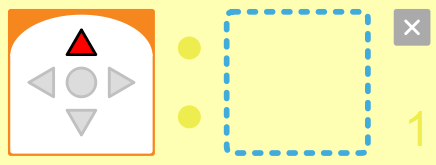
\includegraphics[width=.3\textwidth,keepaspectratio=true]{event-action-pair-yellow1}
&
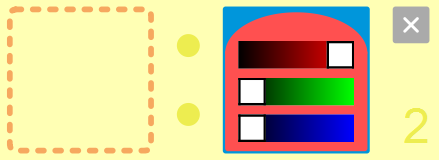
\includegraphics[width=.3\textwidth,keepaspectratio=true]{event-action-pair-yellow2}
\end{tabular}
\end{center}

The left gold-colored square is the space for the event; the right
blue-colored square is for the first (or only) action. The pair with the
yellow background is called the \emph{current} pair.

\informationbox{Quick entering of a block}{If you click on an event or action block, it will be
automatically placed in the program area in the current
event-actions pair.}

\bigskip

\bigskip

\informationbox{The VPL toolbar}{\cref{a.toolbar} contains a
description of all the buttons in the VPL toolbar. Look at it
occasionally until you have learned how to use them.}

\chap{Changer les couleurs}

\sect{Colorer Thymio}

Créons un programme qui affiche deux couleurs différentes sur le dessus de Thymio lorsque les boutons avant ou arrière sont touchés, et deux autres couleurs sous et sur les côtés de Thymio lorsque les boutons gauche ou droite sont touchés.

{\raggedleft \hfill Programme: \bu{colors.aesl}}

Nous avons besoin de quatre paires d'événement-action.
Il y a quatre événements --- toucher l'un des quatre boutons --- et une action couleur est associée avec chaque événement.
Notez la différence entre le bloc \blksm{action-colors-up-white} et le bloc \blksm{action-colors-down-white}. Le premier des deux change la couleur affichée sur le dessus de Thymio alors que le deuxième change la couleur affichée sur le dessous et sur les côtés. Le deuxième bloc a deux marques noires qui représentent les roues du robot.

Ce programme est illustré sur la \cref{fig.colors-a}.

Quelles couleurs seront affichées? Pour les premières trois actions, le slider d'une couleur a été glissé tout à droite alors que les autres sont restés à gauche.
Ces actions affichent donc respectivement purement du rouge, du bleu et du vert.
L'action associée avec le bouton gauche mixe du rouge et du vert, ce qui produit donc du jaune.
Vous pouvez voir que le fond de l'action couleur se colorie en fonction de la position des \textit{sliders}, cela vous montre de quelle couleur sera Thymio!

Lancez le programme (icône \blksm{run}) et vérifiez que toucher les boutons change les couleurs du robot.
La \cref{fig.front} montre Thymio illuminé en rouge sur le dessus et la \cref{fig.bottom} montre Thymio illuminé en vert sur le dessous.

\exercisebox{\thechapter.1}{
Expérimentez avec les sliders pour voir quelles couleurs peuvent être affichées.
}

\sect{Éteindre les lumières}

Modifions maintenant le programme pour que les lumières s'éteignent lorsque le bouton central est touché. Nous allons avoir besoin de deux paires événement-action, une pour éteindre les lumières du dessus de Thymio et une autre pour les lumières du dessous. En faisant glisser tous les \textit{sliders} sur la gauche, comme sur la \cref{fig.colors-b}, la lumière sera éteinte.
Vous voyez que l'événement est le même, toucher sur le bouton central, mais l'action associée est différente, éteindre les lumières du haut ou du bas.
N'oubliez pas de lancer le programmer en cliquant sur l'icône \blksmpure{run}.
À l'avenir, il sera implicite qu'il vous faudra lancer chaque programme en cliquant sur cet icône, nous ne vous le dirons plus.

\vfill


\importantbox[De multiples paires événement-action]{
\begin{itemize}[noitemsep,nosep,leftmargin=*]
\item Lorsqu'un programme est lancé, toutes les paires d'événement-action sont actives.
\item Il est possible d'avoir plusieurs fois le même événement mais il faut que le bloc d'action associé soit différent.
\item Si l'événement et le bloc d'action sont identiques dans plusieurs paires, VPL vous indiquera qu'il y a une erreur (zone 3 dans la \cref{fig.vplgui}). 
Vous ne pourrez pas lancer le programme tant qu'il y a des erreurs.
\end{itemize}
}

\begin{figure}
    \centering
    \subfigure[Changer les couleurs lorsqu'un bouton flèche est touché]{
		\label{fig.colors-a}
		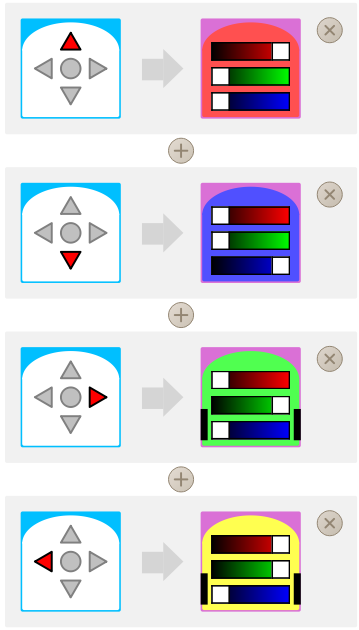
\includegraphics[width = 0.4\textwidth]{colors1}
	}
    \hspace{1.5cm}
    \subfigure[Éteindre Thymio lorsque le bouton centrale est touché]{
		\label{fig.colors-b}
		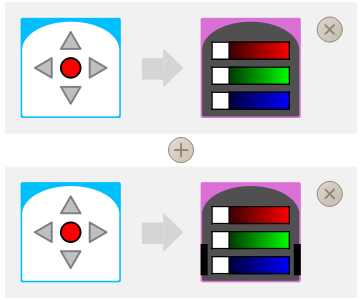
\includegraphics[width = 0.4\textwidth]{colors2}
	}
    \caption{Jouer avec les lumières de Thymio}
    \label{fig.colors}
\end{figure}

\chap{Los, Thymio-II bewege dich}\label{c.moving}

\sect{Vorwärts und Rückwärts fahren}

Der Thymio-II Roboter hat zwei Motoren mit denen er seine zwei Räder antreiben
kann. Beide Motoren können vorwärts und rückwärts drehen. Dadurch kann der
Roboter vorwärts und rückwärts fahren. Lass uns ein kleines Projekt machen, mit
dem du lernen kannst, wie du die Motoren steuern kannst.

Der Aktions-Block für die Motoren \blk{action-motors} zeigt ein kleines Bild
des Roboters in der Mitte und zwei Balken. Mit den beiden Balken kannst du die
Geschwindigkeit der beiden Motoren einstellen. Mit dem linken Balken die des
linken Motors und mit dem rechten Balken die des rechten Motors. Wenn das
weisse Quadrat in der Mitte ist, dreht der Motor nicht. Wenn du das Quadrat
nach oben schiebst, dreht der Motor immer schneller vorwärts. Schiebst du es
nach unten, dreht der Motor rückwärts.

Konstruiere ein Programm, um den Roboter vorwärts fahren zu lassen, wenn der
Vorwärts-Kopf berührt wird und rückwärts, wenn der Rückwärts-Knopf berührt
wird.

{\raggedleft \hfill Beispielprogramm \bu{moving.aesl}}

Wir brauchen zwei Ereignis-Aktions-Paare (Bild~\ref{fig.nostop}). Erstelle die
beiden Paare und stelle bei den Motoren die gleiche Geschwindigkeit ein.

Führe das Programm aus, indem du auf \blksm{run} klickst. Jetzt kannst du den
Vorwärts- und Rückwärts-Knopf berühren. Was macht der Roboter?

\begin{figure}
\begin{center}
\gr{no-stop-motors}{.4}
\caption{Vorwärts und rückwärts fahren}\label{fig.nostop}
\end{center}
\end{figure}

\sect{Stoppe den Roboter}

\textbf{Hilfe!} Ich kann den Roboter nicht mehr stoppen!

Klicke auf das Symbol \blksm{stop}, um den Roboter zu stoppen.

Wie können wir dieses Problem beheben? Lass uns ein neues Ereignis-Aktions-Paar
hinzufügen, das beide Motoren stoppt, wenn du den mittleren Knopf berührst.
Hier musst du beim Aktions-Block für die Motoren die Balken in der Mitte
lassen.

\sect{Falle nicht vom Tisch}

Wenn der Roboter auf dem Boden fährt, kann er im schlimmsten Fall in eine Wand
fahren, oder sein USB Kabel ausziehen. Aber wenn der Roboter auf einem Tisch
fährt, kann er auf den Boden fallen und kaputt gehen! Lass uns den Roboter so
programmieren, dass das nicht passieren kann.

\centeredbox{\textbf{Achtung! Wenn der Roboter auf einem Tisch fährt, musst du
bereit sein, um ihn aufzufangen falls er runter fällt.}}

Drehe deinen Thymio-II auf den Rücken. Nun siehst du, dass er unten zwei
kleine, schwarze Rechtecke mit optischen Elementen hat (Bild~\ref{fig.bottom}).
Das sind \emph{Bodensensoren}, die Licht aussenden, und erkennen können, ob
viel oder wenig Licht zurückkommt. Wenn etwas unter dem Roboter ist (zum
Beispiel der Tisch) wird viel Licht reflektiert. Wenn aber die Spitze des
Roboters über den Tisch hinausragt, geht das Licht weit weg und nur sehr wenig
kommt zurück. Wenn das passiert, möchten wir den Roboter stoppen.

\centeredbox{\textbf{Hier nehmen wir an, das dein Tisch eine helle Farbe hat.
Wenn du einen sehr dunklen Tisch hast, musst du das Programm ändern.}}

Ziehe das Bodensensor-Ereignis \blk{event-ground} in dein Programm. Oben hat
dieser Block zwei kleine Quadrate. Wenn du sie anklickst, werden sie weiss, rot
und dann wieder grau. Die Farben haben verschiedene Bedeutungen:

\begin{itemize}
\item \textbf{Grau}: Der Sensor wird nicht gebraucht.
\item \textbf{Rot}: Ein Ereignis passiert, wenn viel Licht reflektiert wird.
\item \textbf{Weiss}: Ein Ereignis passiert, wenn wenig Licht reflektiert wird. 
\end{itemize}

Klicke auf die Quadrate bis beide weiss sind, um den Roboter zu stoppen, wenn
wenig Licht reflektiert wird. Erstelle so das Ereignis-Aktions-Paar
\blk{dont-fall}.

\begin{figure}
\begin{center}
\gr{bottom}{0.6}
\caption{Unten hat der Thymio-II Roboter zwei Bodensensoren.}\label{fig.bottom}
\end{center}
\end{figure}

Stelle den Roboter nahe an die Tischkante und berühre den Vorwärts-Knopf. Der
Roboter sollte bis zur Tischkante fahren und dann stoppen.

Als ich das Programm ausprobiert habe, ist der Roboter heruntergefallen. Das ist
passiert, weil mein Tisch eine runde Kante hat. Als der Roboter die Kante
richtig bemerkt hat, war es schon zu spät und er ist runter gefallen. Ich habe
ein Stück schwarzes Klebeband an die Tischkante geklebt, damit hat es dann
funktioniert.

\sect{Aufgabe \thechapter.1}

Probiere verschiedene Geschwindigkeiten mit dem Roboter aus. Kann der Roboter
auch bei der schnellsten Geschwindigkeit noch rechtzeitig stoppen, um nicht vom
Tisch zu fallen? Falls nicht, wie schnell kannst du ihn einstellen, damit er
noch rechtzeitig stoppen kann?


\chap{Un robot de compagnie}\label{ch.pet}

Un \emph{robot autonome} adopte un comportement spécifique en fonction de la situation dans laquelle il se trouve.
Il réussi à réagir grâce au \textit{feedback}, littéralement de l'information en retour.
Il faut donc que le robot puisse «\,voir\,» le monde qui l'entoure pour pouvoir y réagir.

\sect{Thymio vous obéit}

Pour commencer, nous allons programmer Thymio pour qu'il vous obéisse.
Normalement, le robot restera sur place sans bouger ; quand il détectera votre main devant lui, il bougera en sa direction.

Thymio a cinq capteurs de distance horizontaux à l'avant et deux à l'arrière.
Ils sont similaires à ceux qui se trouve sous Thymio et que nous avons utilisé au \cref{c.moving}.
Avancez votre main en direction des capteurs à l'avant de Thymio, vous verrez une lumière rouge apparaître à côté du capteur qui vous aura détecté, comme sur la \cref{fig.detect}.

\begin{figure}
\begin{center}
\gr{detect}{.6}
\caption{L'avant de Thymio. Deux doigts sont détectés par les capteurs. avant.}\label{fig.detect}
\end{center}
\end{figure}

Le bloc \blksm{event-prox} sert à utiliser les capteurs horizontaux avants et arrières de Thymio.
Les petits carrés gris (cinq sur l'avant et deux sur l'arrière) sont utilisées comme pour les détecteurs situés sous Thymio.
En cliquant dessus, ils passent de gris à blanc, à rouge et à nouveau à gris.
Pour ce bloc, les significations des couleurs sont :

\begin{itemize}
\item \textbf{Gris} : Le détecteur n'est pas utilisé.
\item \textbf{Rouge} : L'événement associé est déclenché si un objet se trouve proche.
\item \textbf{Blanc} : L'événement associé est déclenché si aucun objet ne se trouve proche.
\end{itemize}

\importantbox[Détecteurs de sols et capteurs de distance horizontaux]{
Attention à ne pas confondre le comportement des capteurs de distance horizontaux avec celui des détecteurs de sols.
\begin{itemize}[noitemsep,nosep,leftmargin=*]
\item Pour les capteurs horizontaux, le carré blanc spécifie qu'un événement se produire s'il n'y a \emph{rien à proximité}, alors qu'un carré rouge spécifie qu'un événement se produira s'il y a \emph{quelque chose à proximité}.
\item Pour les détecteurs de sols, le carré blanc spécifie qu'un événement se produira s'il y a \emph{peu de lumière réfléchie par la surface} alors qu'un carré rouge spécifie qu'un événement se produira \emph{s'il y a beaucoup de lumière réfléchie par la surface}.
\end{itemize}
Le principe physique de ces deux types de capteurs est similaire, mais parce qu'ils sont placés différemment, leur comportement est différent.
}

Pour construire le comportement, il nous faut deux paires événement-action, comme sur la \cref{fig.follow-hand}.
Dans ce programme, vous voyez que dans la première paire, le carré central est blanc et l'action associée est que les moteurs sont arrêtés.
Ainsi, lorsque le robot ne voit rien, il ne bougera pas ; et s'il bougeait, il s'arrêtera.
Dans la deuxième paire, le carré central est rouge et les sliders du bloc action moteur sont glissés vers le haut.
Ainsi, lorsque vous amenez votre main près de l'avant du robot, un événement se produit qui fait tourner les deux moteurs assez vite et fait avancer le robot en avant.


\begin{figure}
\begin{floatrow}
	\ffigbox
	{\caption{Thymio avance vers votre main}\label{fig.follow-hand}}
	{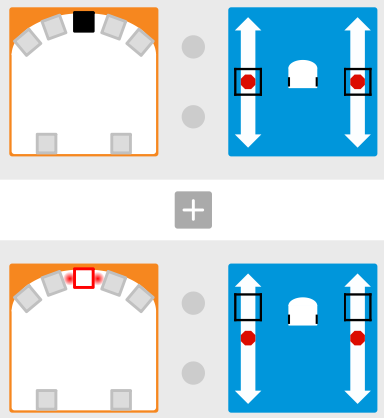
\includegraphics[width=.4\textwidth]{likes-forward}}
	\ffigbox
	{\caption{Un bulldozer à chenilles}\label{fig.bull}}
	{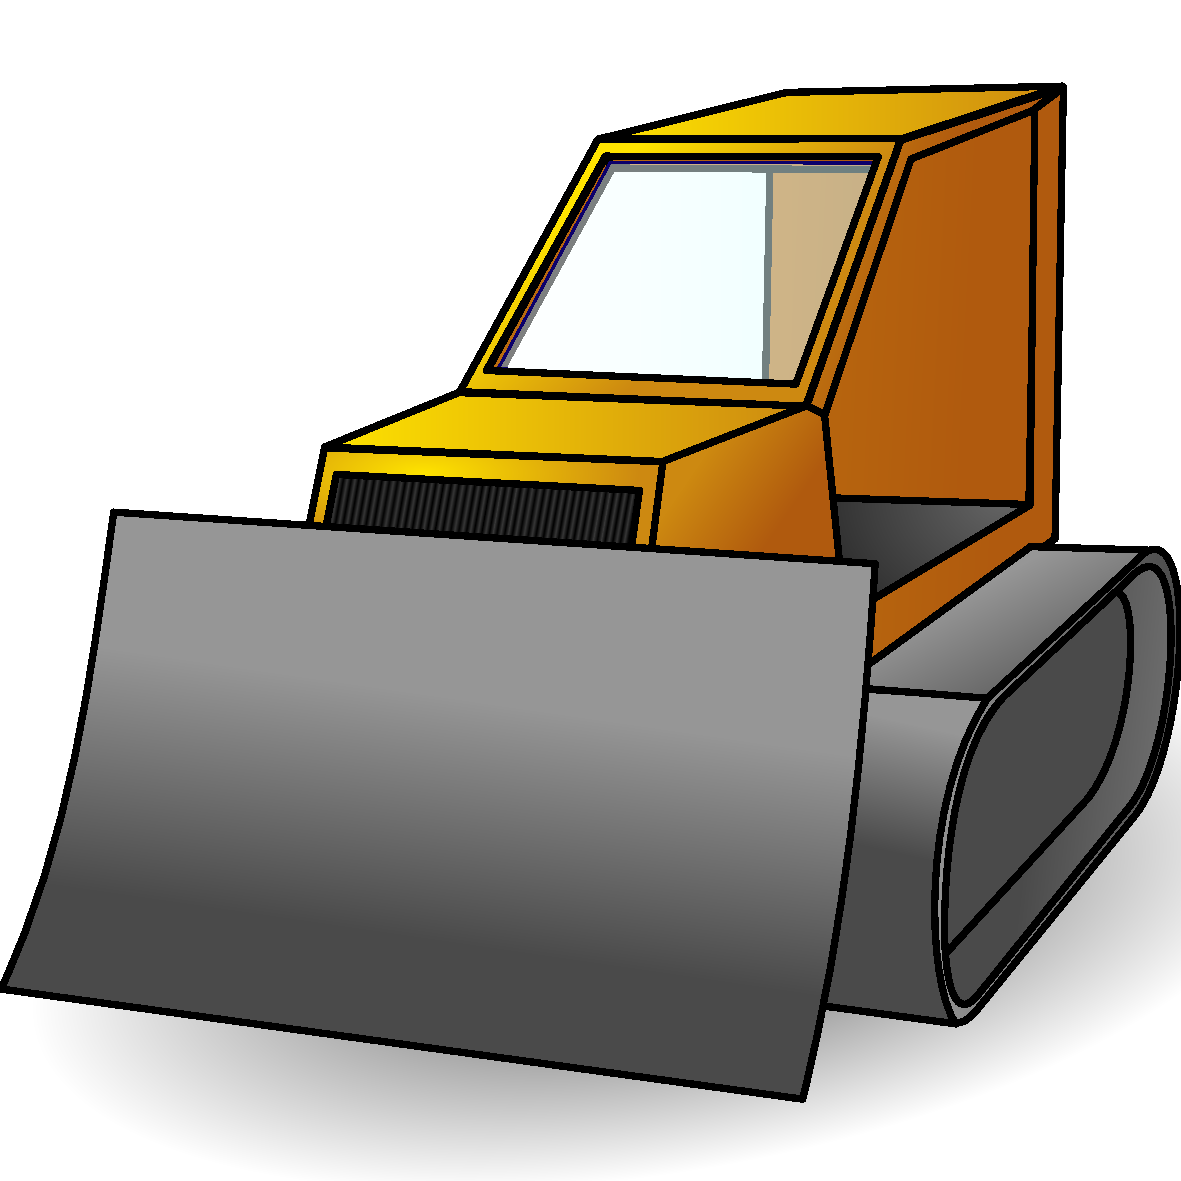
\includegraphics[width=.35\textwidth]{bulldozer}}
\end{floatrow}
\end{figure}

\sect{Faire tourner Thymio}

Thymio n'a pas un volant comme une voiture ou un guidon comme un vélo.
Comment tourne-t-il donc ? 
Pour tourner, le robot utilise une \emph{direction différentielle}, ou \emph{differential drive}, qui est  utilisée par de nombreux véhicules à chenilles comme le bulldozer sur la \cref{fig.bull}.
À la place de tourner un guidon dans la direction désirée, les chenilles ou roues gauches et droites sont commandées par des moteurs individuels à des vitesses \emph{différentes}.
Si la roue droite tourne plus vite que la roue gauche, alors le véhicule tournera à gauche, tandis que si sa roue gauche tourne plus vite que sa roue droite, il tournera à droite.

Dans VPL, en réglant le bloc action moteur avec les \textit{sliders} à des endroits différents, les roues de Thymio ne tourneront pas à la même vitesse, ce qui fera tourner le robot.
Plus la différence de vitesse est élevée, plus le virage sera serré.
Pour arriver à une grande différence de vitesses, vous pouvez faire tourner une roue en avant et l'autre en arrière.
En fait, pour tourner sur lui-même, il suffit à Thymio de faire tourner ses deux roues à la même vitesse mais dans des sens opposés !
Par exemple, dans ce bloc action moteur \blksm{differential}, le \textit{slider} gauche indique une grande vitesse en arrière, alors que le \textit{slider} droite indique une grande vitesse en avant.
Le résultat est que le robot tournera sur lui-même en direction de la gauche, comme indiqué par l'image du robot.

Expérimentez avec une paire événement-action telle que celle ci : \blkc{turning}

Si vous chargez ensuite ce programme et appuyez sur le bouton central, Thymio devrait tourner sur lui-même. Vous pouvez toujours l'arrêter en appuyant sur \blksm{stop}.

\trickbox{L'icône du Thymio au centre du bloc action moteur s'anime dès que vous réglez les \textit{sliders} pour vous donner une idée du mouvement de Thymio!}


\sect{Thymio vous aime}

Un vrai animal de compagnie ne se contente pas de s'approcher ou de s'éloigner de vous, il vous suit un peu partout! 
Pour que Thymio puisse vous suivre le plus fidèlement possible, il faudra ajouter deux paires événement-action au programme précédant.
Si Thymio vous détecte avec son capteur avant-droit, il doit tourner à droite et s'il vous détecte avec son capteur avant-gauche, il doit tourner à gauche.

{\raggedleft \hfill Programme \bu{likes.aesl}}

Une façon de faire est illustrée sur la \cref{fig.likes}.
Vous pouvez essayer différentes vitesses, le faire tourner sur lui-même ou non, afin de trouver le meilleur comportement !

\begin{figure}
	\subfigure[Thymio s'oriente face à vous]{
		\label{fig.likes}
		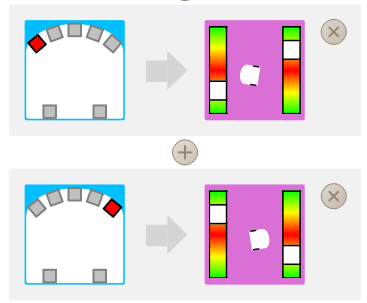
\includegraphics[width=.4\textwidth]{likes-turns}
	}
	\hfill
	\subfigure[Thymio vous évite]{
		\label{fig.hates}
		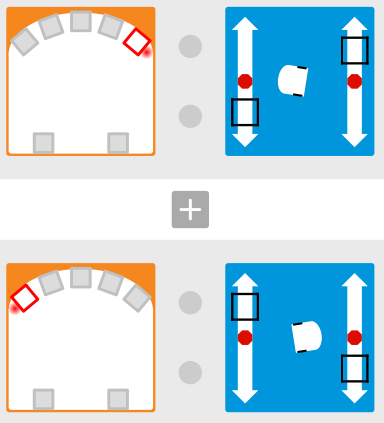
\includegraphics[width=.4\textwidth]{hates}
	}
	\caption{Programmes pour robot de compagnie}
\end{figure}

\exercisebox{\thechapter.1}{
Modifiez le comportement du robot de compagnie pour qu'il bouge en avant quand le programme est exécuté et qu'il s'arrête lorsqu'il détecte le bord de la table (ou une bande de ruban adhésif noir). \\
{\small Comme vu dans le \cref{c.moving}, beaucoup de lumière sera réfléchie par une surface blanche, et peu par une surface noire.
Vous aller devoir expérimenter avec le bloc capteurs horizontaux pour déterminer quand choisir un carré blanc et quand choisir un carré noir, en fonction du sol ou de la table sur lequel vous placez le robot.}
}

\exercisebox{\thechapter.2}{
Qu'arrive-t-il si vous changez l'ordre des paires d'événement-action utilisées à l'exercice précédent ?
}


\sect{Thymio ne vous aime pas}

Parfois, même le plus fidèle animal de compagnie n'a pas envie de vous suivre. 
Écrivez un programme qui génère ce comportement.

{\raggedleft \hfill Programme \bu{does-not-like.aesl}}

Ouvrez le programme du Thymio qui vous aime et inversez l'association des événements avec les actions, comme montré sur la \cref{fig.hates}.
Détecter un obstacle avec le capteur gauche fait tourner le robot à droite, et détecter un obstacle avec le capteur droite fait tourner le robot à gauche.

% \begin{figure}[h]
%     \centering
%     \subfigure[S'il vous détecte devant lui, il recule]{ \label{fig.recule} 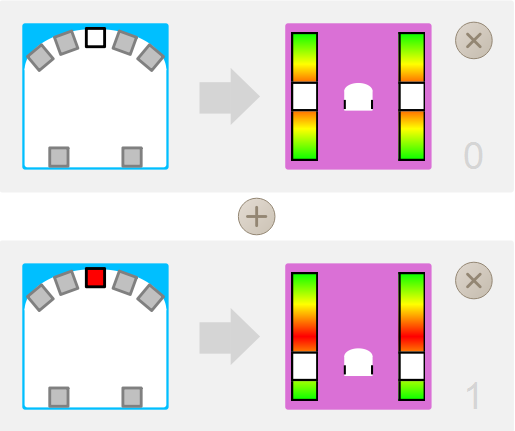
\includegraphics[width = 0.35\textwidth]{hates2}}
%     \hspace{1cm}
%     \subfigure[S'il vous détecte sur les côtés, il vous évite]{ \label{fig.evite} 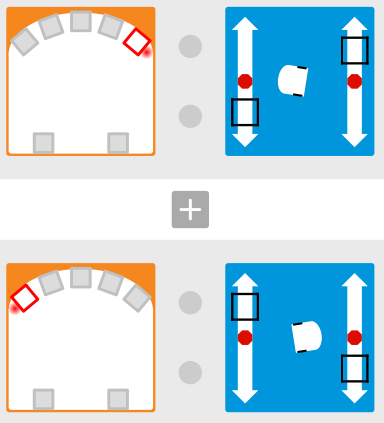
\includegraphics[width = 0.35\textwidth]{hates}}
%     \caption{Thymio vous évite et vous fuit}
%     \label{fig.recule-evite}
% \end{figure}

\exercisebox{\thechapter.3}
{
Jouez avec les différents capteurs avant de Thymio.
Les capteurs horizontaux avant sont numérotés 0, 1, 2, 3, 4 de gauche à droite.
Les capteurs arrière sont numérotés 5 pour le gauche et 6 pour le droite.
À la place d'utiliser les capteurs 0 et 4 comme jusqu'à maintenant:
\begin{itemize}[noitemsep,nosep,leftmargin=*]
\item Utilisez les capteur 1 pour tourner le robot à gauche et le 3 pour à droite.
\item Utilisez à la fois les capteurs 0 et 1 pour tourner le robot à gauche et à la fois les capteurs 3 et 4 pour tourner le robot à droite.
\item Ajouter une paire événement-action pour les capteurs arrières 5 et 6.
\end{itemize}
}

\sect{Régler les \textit{sliders} plus précisément (avancé)}

Ce n'est pas très facile de régler les \textit{sliders} précisément pour, par exemple, faire avancer Thymio tout droit.
En regardant la traduction textuelle des paires événement-action, il est possible d'ajuster plus précisément les vitesses des roues.
Le \cref{fig.textcode} montre le programme du Thymio qui vous suit, avec la traduction texte à droite.
Ce texte est écrit automatiquement quand vous éditez les paires événement-action.

\begin{figure}
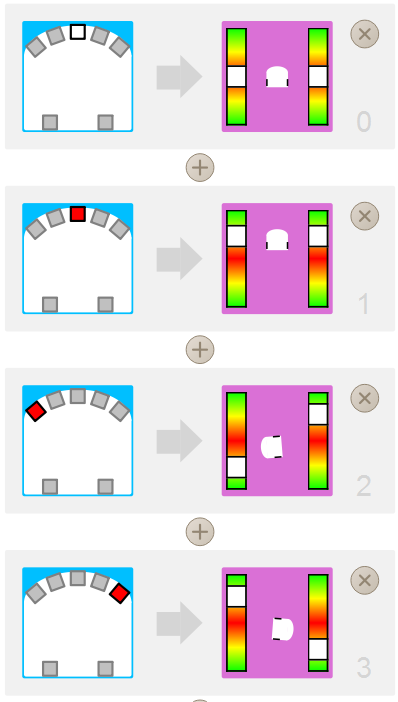
\includegraphics[width=0.3\textwidth]{follow4}
\hfill
\begin{minipage}[b]{0.6\textwidth}
\footnotesize
\begin{lstlisting}
onevent prox
	if prox.horizontal[2] < 400 then
		motor.left.target = 0
		motor.right.target = 0
	end
	if prox.horizontal[2] > 500 then
		motor.left.target = 300
		motor.right.target = 300
	end
	if prox.horizontal[0] > 500 then
		motor.left.target = -300
		motor.right.target = 300
	end
	if prox.horizontal[4] > 500 then
		motor.left.target = 300
		motor.right.target = -300
	end
\end{lstlisting}
\end{minipage}
\caption{Un programme VPL et le programme texte correspondant.}
\label{fig.textcode}
\end{figure}

La ligne \p{onevent prox} signifie que les lignes qui suivent seront exécutées lorsque la lecture des capteurs de distance (appelés \textit{proximity} et abrégés \textit{prox}) se produit (elle se produit 10 fois par seconde).

Lorsque l'événement se produit, Thymio teste la valeur des capteurs en utilisant une condition de type \p{if} \ldots \ \p{then} \ldots \ \p{end}, c'est à dire \p{si} \ldots \ \p{alors} \ldots \ \p{fin}.
Il commence par tester le capteur numéro 2 (avant centre) comme nous le voyons avec \p{prox.horizontal[2]}.
Si cette valeur est inférieure à 400, alors Thymio règle la vitesse des moteurs gauche et droite à 0 avec les instructions \p{motor.left.target = 0} et \p{motor.right.target = 0}.
Chaque bloc \p{if} \ldots \ \p{then} \ldots \ \p{end} teste un capteur spécifique et effectue ou non l'action associée, en fonction du résultat du test.
Il correspond donc à une paire événement-action:
\begin{enumerate}[start=0]
	\item teste si rien ne se trouve devant ; si c'est le cas, Thymio s'arrête.
	\item teste s'il y a quelque chose devant ; si c'est le cas, Thymio avance.
	\item teste s'il y a quelque chose à gauche ; si c'est le cas, Thymio tourne à gauche.
	\item teste s'il y a quelque chose à droite ; si c'est le cas, Thymio tourne à droite.
\end{enumerate}
Finalement, une fois que Thymio a testé tous ces capteurs, il attend le prochain événement \p{prox} et recommence ces tests, indéfiniment.
Pour apprendre comment éditer le mode texte, voir le \cref{c.next}.

\trickbox{En bougeant les \textit{sliders} des blocs d'action moteur, vous verrez les vitesses visées pour les moteurs (\p{moter.X.target}) changer par pas de 50 dans l'intervalle $-$500 à 500.
En bougeant les \textit{sliders} avec soin, vous pouvez choisir n'importe laquelle de ces valeurs.
}
% !TeX root = vpl.tex

\chap{The Robot Finds Its Way by Itself}\label{ch.line}

Consider a warehouse with robotic carts that bring objects to a central
dispatching area. There are lines painted on the floor of the warehouse
and the robot receives instructions to follow certain lines until it
reaches the storage bin of the desired object. Let us write a program
that causes the robot to follow a line on the floor.

{\raggedleft \hfill Program file \bu{follow-line.aesl}}

The line-following task brings out all the uncertainty of constructing
robots in the real world: The robot must deal with uncertainty in its
perceptions and its actions. For instance, the line might not be
perfectly straight, dust may obscure part of the line, or dirt may cause
one wheel to move more slowly than the other one. To follow a line, the
robot must use a \emph{controller} that decides how much power to apply
to each motor depending on the data received from the sensors.

\sect{The line and the robot}

To follow a line, we use the ground sensors (\cref{ch.moving}). Remember
that these work by sending infrared light (which is invisible to human
eye) and measuring how much is reflected back. If the floor is
light-colored, the sensor will detect a lot of reflected light and the
event \blksm{lots-of-light} will occur. We need a line that will cause
an event to occur when there is little reflected light
\blksm{little-light}. This is easy to do by printing a black line on
paper and taping it to the floor, by painting the line, or by sticking
black electrician's tape on the floor (\cref{fig.tape}). The line must
be wide enough so that both ground sensors will sense black when the
robot is successfully following the line. A width of 5 centimeters is
sufficient for the robot to follow the line even if there are small
deviations.

\begin{figure}
\subfigure[Thymio following a line of tape]%
{\label{fig.tape}%
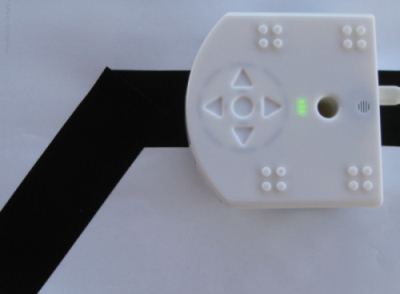
\includegraphics[height=0.35\textwidth]{blacktape}}
\hfill
\subfigure[The left sensor is off the tape and the right sensor is on the tape]%
{\label{fig.one-off}%
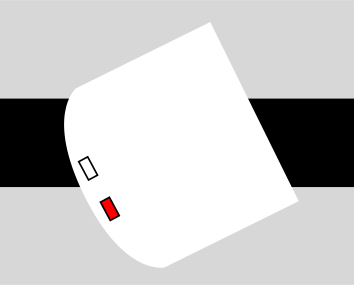
\includegraphics[height=0.35\textwidth]{thymio_half_on_line}}
\caption{Thymio on a black tape}
\end{figure}

To implement line-following, first, we cause the robot to move forward
whenever \emph{both} sensors detect a dark surface (it is on the line)
and to stop whenever \emph{both} sensors detect a light surface (it is
not the line):

The event-actions pairs are shown in \cref{fig.start-stop}.
                  
\begin{figure}
\subfigure[Start and stop the robot]%
{\label{fig.start-stop}%
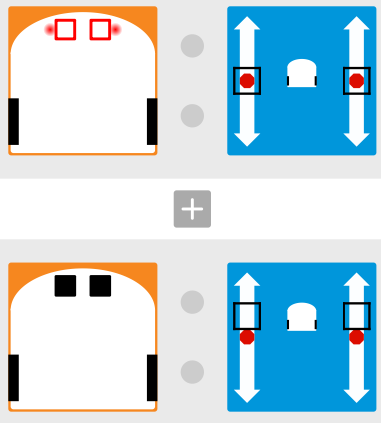
\includegraphics[width=0.4\textwidth]{line-forward}}
\hfill
\subfigure[Correcting deviations]%
{\label{fig.follow-line}%
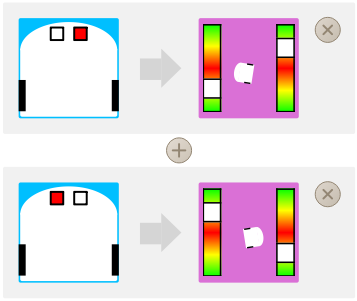
\includegraphics[width=0.4\textwidth]{line-controller}}
\caption{A program for line following}
\end{figure}

%\begin{center}
%\begin{tabular}{cc}
%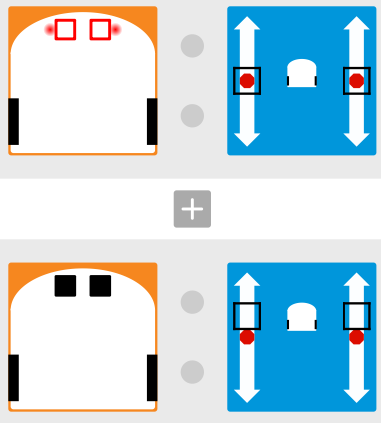
\includegraphics[width=0.4\textwidth]{line-forward} &
%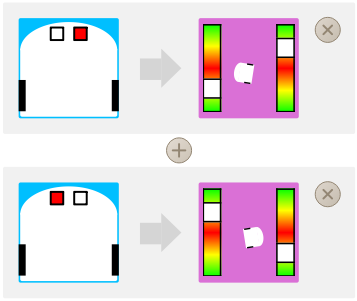
\includegraphics[width=0.4\textwidth]{line-controller} \\
%(a) Start and stop the robot & (b) Follow the line \\
%\end{tabular}
%\end{center}

\trickbox{Make sure that you use a USB cable that is long enough (say,
two meters), so that the Thymio can stay connected to the computer even
as it moves. You can find extension cables in any computer shop.}

\sect{Your first controller}

The next step is to program the controller that follows the line. Two
event-actions pairs are needed, as shown on the image above (b):

\begin{itemize}

\item If the robot moves off the tape to the \emph{left}
(\cref{fig.one-off}), the \emph{left} sensor will detect the floor while
the \emph{right} sensor is still detecting the tape; in that case the
robot should turn slightly to the \emph{right}.

\item If the robot moves off the tape to the \emph{right}, the
\emph{right} sensor will detect the floor while the \emph{left} sensor
is still detecting the tape; in that case the robot should turn slightly
to the \emph{left}.

\end{itemize}

%Two event-actions pairs are needed, as shown in \cref{fig.follow-line}.

\sect{Setting the parameters}

It is easy to see that if the robot runs off the left edge of the tape,
it has to turn to the right (\cref{fig.one-off}). The question is
how tight should the turn be? If the turn is too gentle, the right
sensor might \emph{also} run off the tape before the robot turns back;
if the turn is too aggressive, it might cause the robot to run off the
other end of the tape. In any case, aggressive turns can be dangerous to
the robot and whatever it is carrying.

You will need to experiment with the speeds of the left and right motors
in each motor action block until the robot runs \emph{reliably}. Here,
reliably means that the robot can successfully follow the line several
times. Since each time you place the robot on the line you might place
it at a slightly different position and point in a slightly different
direction, you need to run several tests to make sure that the program
works.

There are many ways to configure the motor action blocks. The forward
speed of the robot on the line is an important parameter. If it is too
fast, the robot can run off the line before the turning actions can
affect its direction. However, if the speed is too slow, no one will buy
your robot to use in a warehouse.

If the robot starts to leave the line, what should it do? If it makes a
sharp turn (one motor goes forward and the other backwards), the robot
will return quickly to the line, but its movements will be very jerky.
On the other hand, if the robot makes a gentle turn (one motor goes
slightly faster than the other), the robot will move smoothly but it may
lose the line. You will have to experiment to find good compromises.

\newpage

\exercisebox{\thechapter.1}{The robot stops when both ground sensors
detect that they are off the tape. Modify the program so that the robot
makes a gentle left turn in an attempt to find the tape again. Try it on
a tape with a left turn like the one shown in \cref{fig.tape}. Try
increasing the forward speed of the robot. What happens when the robot
gets to the end of the tape?}

\bigskip

\exercisebox{\thechapter.2}{Modify the program from the previous
exercise so that the robot turns right when it runs off the tape. What
happens?
\vspace{.5em}\\
It would be nice if we could \emph{remember} which sensor was the last
one to lose contact with the tape in order to cause the robot turn in
the correct direction to find the tape again. In \cref{ch.states} we
will learn how Thymio can remember information.}

\bigskip

\exercisebox{\thechapter.3}{
Experiment with different arrangements of the lines of tapes:
\begin{itemize}[noitemsep,nosep,leftmargin=*]
\item Gentle turns;
\item Sharp turns;
\item Zigzagging lines;
\item Wider lines;
\item Narrow lines.
\end{itemize}
Run competitions with your friends: Whose robot successfully follows the
most lines? For each line, whose robot follows it in the shortest time?
}

\bigskip

\exercisebox{\thechapter.4}{
Discuss what effect the following modifications to the Thymio would
have on the ability of the robot to follow a line:
\begin{itemize}[noitemsep,nosep,leftmargin=*]
\item Ground sensing events occur more often or less often than 10 times a second;
\item The sensors are further apart or closer together;
\item There are more than two ground sensors on the bottom of the robot.
\end{itemize}
}

\chap{Glocken und Pfeifen}
\label{ch.bells}

Lass uns eine Pause von den schwierigen Aufgaben,
wie dem folgen einer Linie machen
und etwas Spass mit dem Roboter haben.
Wir zeigen Dir wie:

\begin{itemize}
\item Komponiere Musik für den Roboter
\item Lass den Roboter auf Musik antworten
\item Lass den Roboter antworten, falls er berührt wird.
\end{itemize}

\sect{Spiele Musik}

Der Thymio-II Roboter enthält ein Synthesizer
und Du kannst diesen programmieren,
um einfache Melodien zu spielen,
indem du den Aktionsblock Musik benutzt \blk{action-music}.

{\raggedleft \hfill Program file \bu{bells.aesl}}

Du wirst kein neuer Beethoven werden
- da nur sechs Noten, in fünf Tonlagen und zwei Tonlängen zur Verfügung stehen -
aber Du kannst eine Melodie komponieren, die dein Roboter einzigartig macht. 
Die Figur Figure~\ref{fig.music} zeigt zwei Ereignis-Aktions Paare,
welche mit einer Melodie antworten,
falls der vordere oder der hintere Schalter berührt wird.
Jedem Ereignis ist eine andere Melodie zugeordnet.

\begin{figure}
\begin{center}
\gr{music}{.4}
\caption{Spiele eine Melodie}
\label{fig.music}
\end{center}
\end{figure}

Die kleinen Kreise sind die sechs Noten.
Die weissen Noten sind lange Tonlängen
und schwarze Noten sind kurze Tonlängen.
Klicke auf den Kreis, um die Tonlänge zu ändern.
Die fünf farbigen, horizontalen Balken stehen für die Tonhöhe.
Klicke auf den \emph{Balken} über oder unter dem Kreis, um den Kreis zu bewegen. 
(Versuche nicht die Kreise zu verschieben (drag and drop), es wird nicht funktionieren). 

\sect{Übung \thechapter.1}

Schreibe ein Programm,
das Dir erlaubt eine Morsebotschaft zu verschicken.
Eine Morsebotschaft wird mit langen und kurzen Tönen kodiert.
(\emph{Striche} für lange Töne und \emph{Punkte} für kurze Töne).
Zum Beispiel wird der Buchstabe \emph{V} mit drei Punkten und einem Strich kodiert.


\sect{Kontrolliere deinen Roboter durch Töne}

Der Thymio-II hat ein Mikrofon.
Das Ereignis \blk{event-clap} findet statt,
wenn ein lautes Geräusch aufgenommen wird, wie z.B. Händeklatschen.
Das Ereignis-Aktions Paar \\ \blk{clap} wird die Bodenlichter einschalten,
wenn du in die Hände klatschst.

\centeredbox{In einer lauten Umgebung kann ein Geräusch eventuell nicht als Ereignis verwendet werden,
da durch den hohen Geräuschepegel dauernd Ereignisse ausgelöst werden.}

\sect{Übung \thechapter.2}

Schreibe ein Programm,
dass den Roboter losfahren lässt,
falls Du in die Hände klatschst und den Roboter stoppt,
falls Du auf den Schalter drückst.

Schreibe ein Programm, das umgekehrt funktioniert:
Der Roboter soll losfahren,
falls Du auf den Schalter drückst und stoppen,
falls Du in die Hände klatschst.

\sect{Gute Arbeit Roboter!}

Haustiere machen nicht immer das,
was wir von ihnen verlangen.
Manchmal brauchen sie einen freundschaftlichen Klaps um sie zu ermutigen.
Genau gleich funktioniert das mit deinem Roboter.
Der Thymio-II enthält ein Berührungssensor, welcher ein Ereignis auslöst \blk{event-tap}, falls dem Roboter kurz auf seine Oberseite geklopft wird. So bewirkt zum Beispiel das Ereignis-Aktions Paar \blk{touch}, dass die Lichter angehen, falls auf die Oberseite des Roboters geklopft wird.

Erstelle ein Programm für dieses Ereignis-Aktions Paar
und das Paar\blk{clap}, welches die Bodenlichter angehen lässt,
falls Du in die Hände klatschst.

{\raggedleft \hfill Program file \bu{whistles.aesl}}

Kannst Du nur die Oberlichter anstellen?
Dies ist schwierig, da ein Klaps immer auch ein Geräusch erzeugt,
welches laut genug sein kann, um ebenfalls die Bodenlichter anzustellen.
Mit ein bisschen Übung wird es Dir jedoch möglich sein,
dem Roboter ein so gefühlsvollen Klaps zu geben,
dass das Geräusch kein Ereignis auslöst.

\sect{Übung \thechapter.3}

Schreibe ein Programm, dass den Roboter vorwärts fahren lässt bis er die Wand berührt. 

\textbf{Warnung} Stell sicher, dass der Roboter langsam fährt und sich dadurch nicht selbst beschädigt.

% !TeX root = vpl.tex
\chap{Un tempo per amare}\label{ch.time}

Nel \cref{ch.pet} abbiamo programmato un robot da compagnia a cui piaciamo o non piaciamo.
Consideriamo un comportamento più avanzato: un animale timido che
non può decidersi se gli piaciamo o no. Inizialmente,
l'animale si girerà verso la nostra mano cercando di raggiungerla, ma poi si terrà a distanza. Dopo un po'
cambierà idea e tornerà indietro in direzione
della nostra mano.

{\raggedleft \hfill File di programma \bu{shy.aesl}}

Il comportamento del robot è il seguente. Quando il tasto destro viene toccato il robot gira a destra. Quando rileva la tua mano,
gira a sinistra, ma dopo un po' si rammarica per la sua decisione e gira
indietro. Noi sappiamo come costruire coppie evento-azione per la curva iniziale:
\blkc{start-turn} e per allontanarsi quando viene rilevata la mano:
\blkc{turn-away}

Il comportamento di tornare indietro "dopo un po'" può essere suddiviso in
due parti:

\begin{itemize}

\item \emph{Quando}  il robot inizia ad allontanarsi $\rightarrow$
\emph{avviare un timer} per due secondi.

\item \emph{Quando}  il timer scende a zero $\rightarrow$ \emph{girare}
a destra.

\end{itemize}

Abbiamo bisogno di una nuova \emph{azione} per la prima parte e un nuovo
\emph{evento} per la seconda parte.

L'azione è quella di impostare un \emph{timer}, che è come una sveglia
\blksm{action-timer}. Normalmente, si imposta una sveglia per un tempo assoluto,
ma quando ho impostato la sveglia nel mio smartphone per un tempo assoluto come le ore
7:00, mi dice il tempo relativo: "allarme impostato tra 11 ore e 23
minuti da oggi". Il blocco del timer funziona allo stesso modo: si imposta il
timer per un certo numero di secondi da quando si verifica l'evento e poi l'azione accade. Il timer può essere impostato per un massimo di quattro secondi. Fai clic su
qualsiasi punto all'interno del cerchio nero che rappresenta il quadrante dell'orologio (ma non
sul cerchio nero stesso). Ci sarà una breve animazione e poi
la quantità di tempo fino a quando l'allarme scatta sarà mostrata di colore blu.

\newpage
La coppia evento-azione per questa prima parte del comportamento è:
\blkc{turn-clock}

Il timer è impostato per due secondi. Quando l'evento che rileva la presenza della mano
si verifica, ci saranno due azioni: ruotare il robot di fianco
e l'impostazione del timer.

La seconda parte del comportamento utilizza un evento che si verifica quando l'allarme si spegne,
cioè, quando la quantità di tempo impostato sul timer scende a zero. il blocco dell'evento
 \blksm{event-timer} mostra una sveglia che squilla.

Ecco la coppia evento-azione per fare girare il robot di nuovo a
destra quando il timer scende: \blkc{turn-back}

\exercisebox{\thechapter.1}{
Scrivi un programma che faccia muovere il robot in avanti alla massima velocità per
tre secondi quando il pulsante in avanti viene toccato; quindi corra
all'indietro. Aggiungi una coppia evento-azione per arrestare il robot toccando il
pulsante centrale.
}

\chap{Les états (Mode avancé)}\label{ch.states}

Un programme VPL est composé d'une série de paires événement-actions.
\emph{Tous} les événements sont vérifiés périodiquement et les actions appropriées sont effectuées.
Ceci limite les programmes que nous pouvons créer ; pour aller plus loin nous avons besoin d'une façon de spécifier que certaines paires événement-actions sont actives à un certain moment, alors que d'autres ne le sont pas.

Par exemple, quand Thymio devait suivre une ligne (\cref{ch.line}), lorsque le robot sortait de la ligne, nous aurions aimé qu'il tourne à gauche ou à droite afin de rechercher la ligne dans une direction qui dépendait de quel côté il était sorti.
Pour cela, deux paires événement-actions sont nécessaires:
une pour tourner à gauche lorsque le robot sort à droite de la ligne
et une pour tourner à droite lorsqu'il sort à gauche.

%Les états sont disponibles dans le mode \emph{avancé} de VPL.
%Cliquez sur \blksm{advanced} avant de travailler sur les projets de ce chapitre.

\sect{Tape, tape}

Dans les programmes que nous avons réalisé jusqu'ici, nous avons souvent \emph{démarré} Thymio en appuyant sur un de ces boutons et \emph{arrêté} Thymio en appuyant sur un autre.
Mais regardez votre ordinateur, normalement, il n'a qu'un seul bouton pour l'allumer ou l'éteindre.
%\blksm{power-button} 
Le bouton se \emph{rappelle} s'il est dans l'état \bu{allumé} ou l'état \bu{éteint}.

Écrivons un programme qui allume les lumières du robot si vous lui donnez une petite tape et qui les éteigne si vous lui donnez une seconde tape.

{\raggedleft \hfill Programme \bu{tap-allumé-éteint.aesl}}

Il est pratique de décrire ce comportement en utilisant un \textit{diagramme d'états} :

\begin{center}
\begin{picture}(240,45)
\thicklines
%\put(0,0){\framebox(240,40){}}
\put(20,20){\circle{40}}
\put(0,0){\makebox(40,40){\textsf{éteint}}}
\put(220,20){\circle{40}}
\put(200,0){\makebox(40,40){\textsf{allumé}}}
\put(40,30){\vector(1,0){160}}
\put(0,30){\makebox(240,10){\textsf{tape $\rightarrow$ allumer}}}
\put(200,10){\vector(-1,0){160}}
\put(0,10){\makebox(240,10){\textsf{tape $\rightarrow$ éteindre}}}
\end{picture}
\end{center}

Ce diagramme comprend deux états indiqués par des cercles, \bu{allumé} et \bu{éteint}.
Depuis l'état \bu{éteint}, le robot peut aller dans l'état \bu{allumé} et revenir, mais seulement en suivant les instructions sur les flèches.
Les instructions décrivent quand une transition d'un état à l'autre peut se produire et comment :

\begin{itemize}

\item \emph{Quand} Thymio est dans l'état \bu{éteint} \textbf{\textit{et}} que l'événement \emph{tape} se produit $\rightarrow$ \emph{allumer} le robot \textbf{\textit{et}} aller dans l'etat \bu{allumé}.

\item \emph{Quand} Thymio est dans l'état \bu{allumé} \textbf{\textit{et}} que l'événement \emph{tape} se produit $\rightarrow$ \emph{éteindre} le robot \textbf{\textit{et}} aller dans l'etat \bu{éteint}.

\end{itemize}

L'accent mis sur le mot \textbf{\textit{et}} avant la flèche~$\rightarrow$ signifie que deux conditions doivent être remplies pour que la transition se fasse: (a) le robot doit être dans un certain état et (b) l'événement doit se produire.
Lorsque les deux conditions sont remplies, alors la transition est prise ce qui fait à la fois changer l'état et exécute l'action écrite après la flèche~$\rightarrow$.

Il est important de réaliser que les deux parties de la condition sont indépendantes.
Dans le diagramme ci-dessus (répété ici),
l'événement \emph{tape} apparaît deux fois, mais l'action 
exécutée lorsque cet événement a lieu 
\emph{dépend de l'état du robot}.

\vspace*{-1ex}

\begin{center}
\begin{picture}(240,40)
\thicklines
%\put(0,0){\framebox(240,40){}}
\put(20,20){\circle{40}}
\put(0,0){\makebox(40,40){\textsf{éteint}}}
\put(220,20){\circle{40}}
\put(200,0){\makebox(40,40){\textsf{allumé}}}
\put(40,30){\vector(1,0){160}}
\put(0,30){\makebox(240,10){\textsf{tape $\rightarrow$ allumer}}}
\put(200,10){\vector(-1,0){160}}
\put(0,10){\makebox(240,10){\textsf{tape $\rightarrow$ éteindre}}}
\end{picture}
\end{center}

\vspace*{-1ex}

Dans un même état, différents événements peuvent causer différentes actions et des transitions vers de nouveaux états différents.
Dans le diagramme suivant, toucher le bouton de gauche
dans l'état \textbf{éteint} allume la lumière verte du robot
et passe l'état du robot à \textbf{allumé1},
alors que toucher le bouton droit \textbf{dans le même état}
entraîne une autre action, allumer la lumière rouge,
et un autre changement d'état vers \textbf{allumé2}.

\vspace*{-1ex}

\begin{center}
\begin{picture}(300,80)
\thicklines
%\put(0,0){\framebox(240,80){}}
\put(25,42){\circle{40}}
\put(10,28){\makebox(30,30){\textsf{éteint}}}
\put(280,20){\circle{40}}
\put(265,6){\makebox(30,30){\textsf{allumé2}}}
\put(40,57){\vector(1,0){220}}
\put(280,65){\circle{40}}
\put(265,50){\makebox(30,30){\textsf{allumé1}}}
\put(40,27){\vector(1,0){220}}
\put(0,60){\makebox(295,10){\textsf{bouton gauche $\rightarrow$ s'allumer en vert}}}
\put(0,30){\makebox(295,10){\textsf{bouton droite $\rightarrow$ s'allumer en rouge}}}
\end{picture}
\end{center}

\sect{Implémenter des diagrammes d'états avec des paires événement-actions}

Nous montrons comment \emph{implémenter} le comportement décrit par le diagramme d'état avec des paires événement-actions.
Implémenter signifie construire un programme qui fera ce que le diagramme d'états ci-dessus décrit.
La \cref{fig.turn-on-off} montre le programme.
Regardons maintenant les paires événement-actions une à une.
Le cercle gauche du bloc \blksm{event-tap} est
sélectionné (et s'affiche en rouge) pour indiquer qu'il s'agit d'un bloc pour l'événement tape.

\importantbox[Le bloc tape en mode avancé]{
Le bloc pour l'événement tape est différent en mode avancé
car il permet aussi l'utilistation des événements
accéléromètre comme décrit au \cref{ch.angles}.}

\begin{figure}
    \subfigure[Une tape pour allumer la lumière]{
        \label{fig.turn-on-off1}
        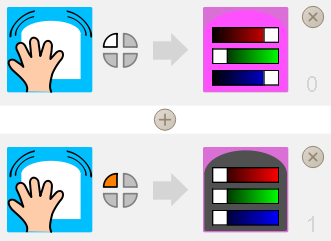
\includegraphics[width=.6\textwidth]{tap-on-off1}
    }
    \subfigure[Une tape pour éteindre la lumière]{
        \label{fig.turn-on-off2}
        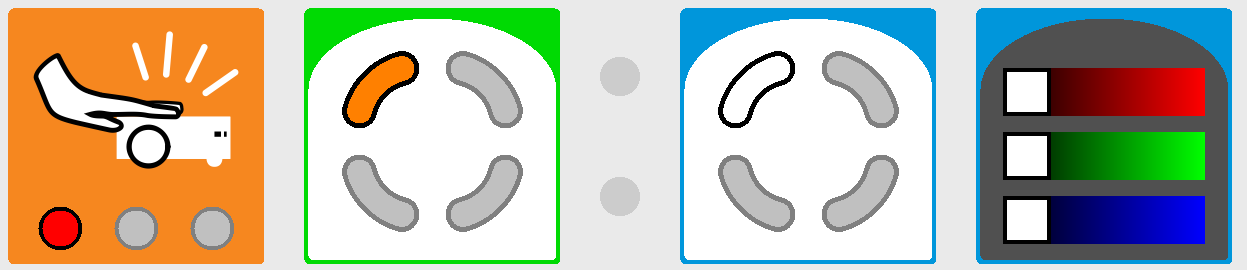
\includegraphics[width=.6\textwidth]{tap-on-off2}
    }
    \caption{Une tape qui a des résultats différents en fonction de l'état.}
    \label{fig.turn-on-off}
\end{figure}

Dans la première paire événement-actions (\cref{fig.turn-on-off1}), l'événement est composé du bloc événement tape avec une indication d'état \blksm{state-filter}.
Un état est indiqué par quatre quartiers d'un cercle, chacun pouvant être soit allumé (orange) ou éteint (blanc).
Dans ce programme, nous utiliserons le quartier en haut à gauche pour indiquer si la lumière du haut du robot est éteinte ou allumée.
Dans \cref{fig.turn-on-off1}, ce quartier est coloré en blanc
et donc la lumière du robot est éteinte.
Ainsi, cette paire veut dire : \textbf{si} le robot est tapé \textbf{et} que le robot est éteint, \textbf{alors} allumer la lumière du robot.

Dans la seconde paire événement-actions
(\cref{fig.turn-on-off2}),
le quartier est coloré en orange et donc la lumière du robot est allumée.
Cette paire veut dire : \textbf{si} le robot est tapé \textbf{et} qu'il est allumé, \textbf{alors} l'éteindre.

Si vous regardez à nouveau le diagramme d'états, vous verrez que seulement la moitié du travail est fait.
En effet, en allumant et éteignant le robot, nous devons aussi changer son état d'\bu{éteint} à \bu{allumé} ou d'\bu{allumé} à \bu{éteint}.
Ainsi, il nous faut ajouter un bloc action \emph{état} \blksm{action-states} à chaque paire.
Ce bloc change l'état selon si les quartiers sont blancs ou oranges.

Pour résumer, la signification du programme de la figure \cref{fig.turn-on-off} est la suivante :

\begin{quote}
    \emph{Quand} le robot est tapé \emph{et} que l'état est \emph{éteint},\\ changer l'état à \bu{allumé} \emph{et} \bu{allumer} la lumière du haut.\\
    \emph{Quand} le robot est tapé \emph{et} que l'état est \bu{allumé},\\changer l'état à \bu{éteint}
    \emph{et} \bu{éteindre} la lumière du haut.
\end{quote}

Chaque événement entraîne à la fois une action lumière et une action état.
Les actions dépendent de l'état dans lequel le robot se trouve, appellé \emph{état actuel}.

\sect{Dans combien d'états différents Thymio peut-il être?}

Quand il est utilisé avec un bloc événement état ou action état, chaque quartier peut être :
\begin{itemize}
	\item \textbf{Blanc}: le quartier est \emph{éteint} ;
	\item \textbf{Orange}: le quartier est \emph{allumé} ;
	\item \textbf{Gris}: le quartier n'est pas pris en compte.
\end{itemize}

Par exemple, dans \blksm{states}, les quartiers en haut à gauche et en bas à droite sont allumés, le quartier en haut à droite est éteint, et le quartier en bas à gauche n'est pas pris en compte.
Ceci veut dire que si \blksmpure{states} est associé à un bloc événement, l'événement se produira si l'état est défini soit par :
\begin{center}
\centering \makebox{\raisebox{-1.7em}{
\includegraphics[height=4em]{states1}}}\quad ou \quad \makebox{\raisebox{-1.7em}{
\includegraphics[height=4em]{states2}}}
\end{center}

Comme chacun des quatre quartiers peut être soit allumé soit éteint, il y a 2 $\times$ 2 $\times$ 2 $\times$ 2 = 16 états :
\begin{quote}
\bu{(éteint, éteint, éteint, éteint)\\(éteint, éteint, éteint, allumé)\\(éteint, éteint, allumé, éteint)\\
\mbox{}\hspace{3em}\ldots\\
(allumé, allumé, allumé, éteint)\\
(allumé, allumé, allumé, allumé)}.
\end{quote}
La \cref{fig.all-states} montre tous les états possibles.
\importantbox{L'état courant du robot est toujours affiché sur le haut du robot par les quatre arcs de cercles lumineux.
Par exemple, la \cref{fig.state-leds} montre le robot dans l'état \bu{(allumé, allumé, allumé, allumé)}.}

\trickbox[Information]{Lorsqu'un programme démarre, l'état initial est toujours 
\bu{(éteint, éteint, éteint, éteint)}:\quad \blkmed{state-all-off}}

\trickbox{Si vous n'utilisez pas tous les 16 états possibles, mais par exemple que 2 ou 4, vous êtes libre de décider quel quartier vous utiliser pour représenter votre état.
Aussi, si par exemple vous avez deux choses différentes à encoder dans l'état, et que chacune d'elle a deux valeurs possibles, vous pouvez utiliser deux quartiers indépendemment.
C'est pourquoi la capacité d'\emph{ignorer} un quartier est très utile !
Essayez toujours de rester le plus simple possible.
}

\begin{figure}
	\subfigure[Tous les états possibles de Thymio]{
		\label{fig.all-states}
		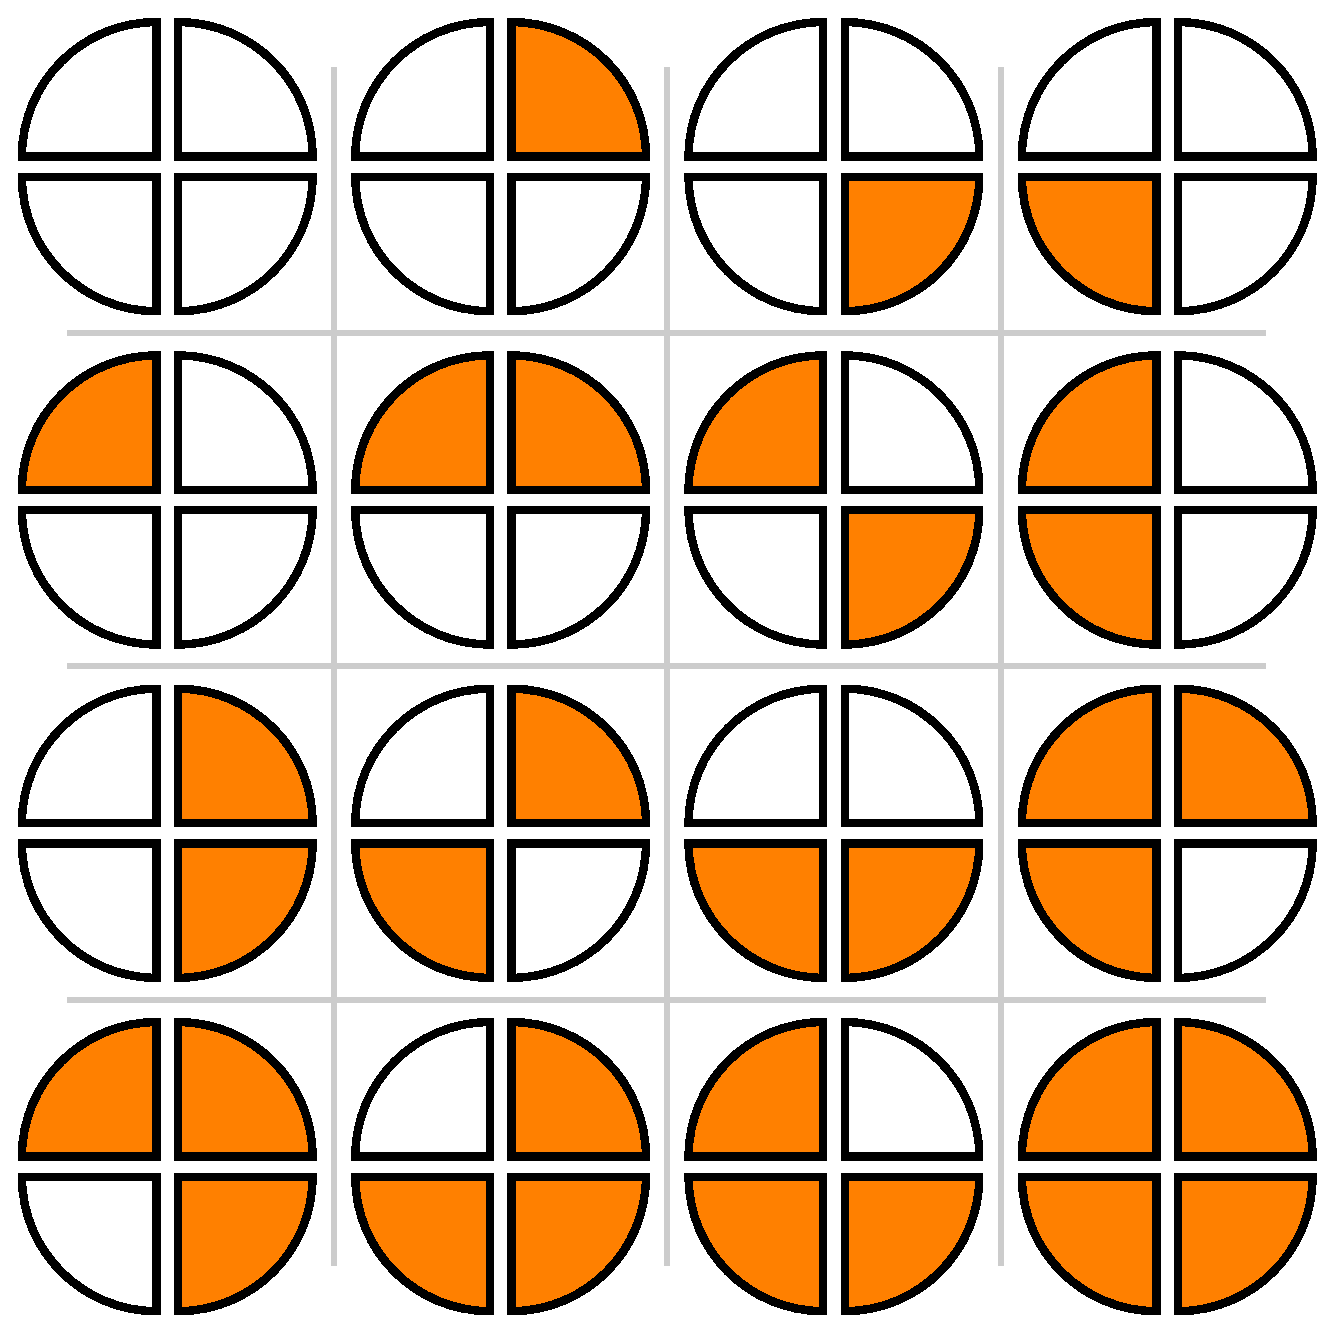
\includegraphics[width = 0.4\textwidth]{all-states}
	} 
	\hfill
        \subfigure[La cercle de lumières indique l'état]{
		\label{fig.state-leds}
		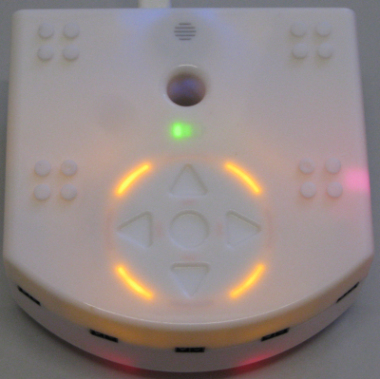
\includegraphics[width = 0.4\textwidth]{state-leds}
	}
	\caption{Les états de Thymio et leur représentation}
\end{figure}

\sect{Attraper la souris}

Écrivons un programme qui fasse tourner le robot de droite à gauche à la recherche d'une souris (ou d'un autre objet).
Si le robot détecte une souris avec son capteur tout à gauche, il continue la recherche jusqu'à ce que la souris soit détectée avec son capteur tout à droite.
Puis, il se positionne en face de la souris, comme sur la \cref{fig.cat-mouse}.

{\raggedleft \hfill Programme: \bu{mouse.aesl}}

Le diagramme d'état suivant décrit le comportement du robot:

\begin{center}
\unitlength=1.2pt
\begin{picture}(320,35)
    %\put(0,0){\framebox(320,35){}}
    \put(40,10){\oval(80,20)}
    \put(160,10){\oval(80,20)}
    \put(280,10){\oval(80,20)}
    \put(0,0){\makebox(80,20){\bu{search left}}}
    \put(120,0){\makebox(80,20){\bu{search right}}}
    \put(240,0){\makebox(80,20){\bu{found}}}
    \put( 80,10){\vector(1,0){40}}
    \put(200,10){\vector(1,0){40}}
    \put(40,35){\vector(0,-1){15}}
\end{picture}
\end{center}

\begin{enumerate}
\item Lorsque le bouton central est touché, le robot entre dans l'état \bu{chercher à gauche} et 
    tourne de droite à gauche.
\item Lorsque le robot est dans l'état \bu{chercher à gauche}
    et détecte la souris sur son capteur tout à droite,
    il prend l'état \bu{chercher à droite} et tourne de gauche à droite.
\item Lorsque le robot est dans l'état \bu{chercher à droite}
    et il détecte la souris avec son capteur central,
    il prend l'état \bu{trouvé} et s'arrête.
\end{enumerate}

L'essentiel est de remarquer que lorsque le capteur central détecte la souris,
le robot s'arrête \emph{seulement si} le robot est dans l'état \bu{chercher à droite}.
Sinon (si la souris est détectée par le capteur central en mode \bu{chercher à gauche}), rien ne se produit.

\begin{figure}
    \begin{center}
        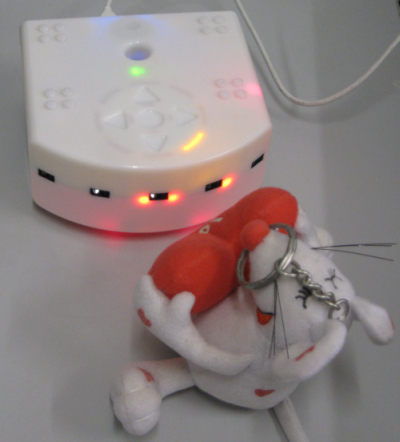
\includegraphics[width=0.4\textwidth]{cat-mouse}
	\caption{Le robot chat cherche la souris}
        \label{fig.cat-mouse}
    \end{center}
\end{figure}

Implémentons ce comportement.
L'état du robot sera défini par le quartier supérieur gauche.
Choisissons le blanc pour représenter l'état \bu{chercher à gauche} et l'orange pour représenter l'état \bu{chercher à droite}.
Puisque le programme se termine lorsque la souris est détectée dans l'état \bu{chercher à droite},
nous n'avons pas besoin de représenter l'état final \bu{trouvé}.
Initialement, tous les quartiers sont \bu{éteints} (blancs).

La paire événement-actions suivante fait tourner le robot à gauche : \blkc{mouse1}
Quand le bouton central est touché, l'état change et devient
\bu{chercher à gauche} \emph{et} le robot tourne à gauche.

%Ceci se produira lorsque le quartier gauche-haut est éteint ; initialement tous les quartiers de l'état sont éteint.

La prochaine paire événement-actions implémente la deuxième étape: \blkc{mouse2}
Quand le robot est dans l'état \bu{chercher à gauche} et
que la souris est détectée par le capteur tout à droite,
l'état devient \bu{chercher à droite}
\emph{et} le robot tourne vers la droite.

Notez que le petit carré à côté de ce capteur est noir pour que l'événement se produise seulement si seul le capteur le plus à droite détecte la souris.

La troisième étape est implémentée dans la paire événement-actions suivante: \blkc{mouse3}
Lorsque la souris est détectée par le capteur central dans l'état \bu{chercher à droite}, le robot s'arrête.


%Pourquoi l'événement de cette paire doit-il dépendre de l'état ?
%La raison est que le capteur central détectera aussi la souris durant le scan initial de droite à gauche.
%Nous voulons que le robot fasse d'abord un scan complet avant de retourner à la position de la souris ; il est donc nécessaire que cette première détection soit ignorée.
%Ceci est accomplit en arrêtant le scan seulement lorsque l'état est \bu{allumé} et ceci arrive que lorsqu'un scan complet a été effectué.

\trickbox{
Il vous faudra expérimenter avec la distance de la souris au robot.
Si elle est trop proche du robot, les capteurs à côte du capteur central détecteront aussi la souris, alors que l'événement demande qu'ils ne la détecte \emph{pas}.
}

\bigskip

\bigskip

\exercisebox{\thechapter.1}{
Écrivez un programme qui fasse danser le robot : il tourne à gauche sur place durant deux secondes, puis tourne à droite sur place durant trois secondes.
Ces mouvement se répètent indéfiniment.
}

\bigskip

\exercisebox{\thechapter.2 (Difficile)}{
Modifier le programme de suivi de ligne du \cref{ch.line} pour que le robot tourne à gauche quand il sort de la ligne par le côté droite, et qu'il tourne à droite quand il sort de la ligne par le côté gauche.
}

\part{From visual to textual programming}

\chap{Learning AESL from VPL programs}\label{ch.next}


Congratulations! You are an expert in programming the Thymio robot using
the \textit{Visual Programming Environment (VPL)}. Now you want to move
on and use the professional \textit{Studio Programming Environment}
(\cref{fig.studio}) and its textual programming language, the
\textit{Aseba Event Scripting Language (AESL)}.

\begin{figure}[hbt]
\begin{center}
\gr{studio}{.9}
\caption{Aseba Studio environment}\label{fig.studio}
\end{center}
\end{figure}

VPL translates graphical programs (event-actions pairs) into a textual
AESL program, which is displayed in the right-hand panel of the VPL
window (panel~6 in \cref{fig.vplgui} on page~\pageref{fig.vplgui}). This tutorial uses VPL programs
from the previous chapters of this tutorial and explains the
corresponding AESL program. You will be able to use your understanding
of the VPL program to learn the fundamental concepts of AESL
programming.

Programming in Aseba Studio is also based upon the concepts of events
and actions. Since VPL programs are translated into AESL programs,
everything you learned in this tutorial is supported in Studio, but now
you have the flexibility of a full programming language with variables,
expressions, and control statements.

When you are working with Aseba Studio, you can open VPL by clicking on
the button \bu{Launch VPL} in the \emph{Tools} tab at the bottom left of
the window. You can import VPL programs into Aseba Studio simply by
opening its file.

Sections marked $^*$ present AESL programming concepts that
go beyond what is found in the VPL projects. They can be skipped when
you first read this tutorial.

\newpage

\textbf{\large Documentation}

To learn about Aseba Studio and AESL, go to the \emph{Programming
Thymio} page at\\
\href{https://www.thymio.org/en:asebausermanual}{https://www.thymio.org/en:asebausermanual}.
You can find documentation of:

\begin{itemize}
\item The Studio programming environment.
\item The AESL programming language.
\item The interface to the Thymio robot.
(There is a reference card for the interface).
\item The native functions library supported in AESL.
\end{itemize}

There is also an archive describing interesting projects in AESL,
together with the source of proposed solutions.

\sect{The Thymio Interface}

Here is the program \p{whistles.aesl} from \cref{ch.bells} together with
part of the corresponding AESL program:
 
\begin{center}
\begin{tabular}{ll}
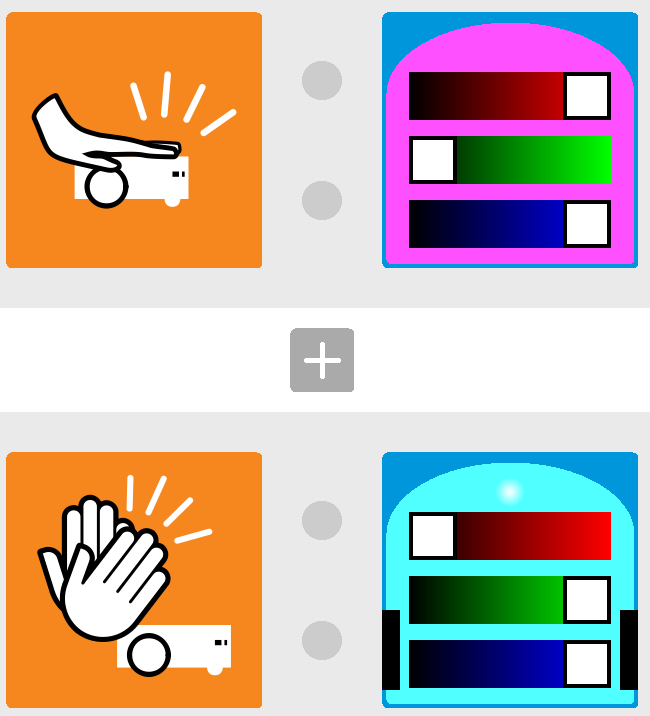
\includegraphics[width=.4\textwidth]{whistles} &
\begin{minipage}[b]{.5\textwidth}
\begin{footnotesize}
\begin{verbatim}
  onevent tap
    call leds.top(32,0,32)
  
  onevent mic
    call leds.bottom.left(0,32,32)
    call leds.bottom.right(0,32,32)
\end{verbatim}
\end{footnotesize}
\vspace*{8ex}
\end{minipage}
\end{tabular}
\end{center}

\textbf{\large Event handlers}

When a tap event occurs, the top light is turned on with the color
called \emph{magenta}, and when the clap event occurs, the bottom light
is turned on with the color called \emph{cyan}. Corresponding to the
event-actions pairs in VPL are \emph{event handlers}, which are
introduced by the keyword \p{onevent} (read this as two words: ``on
event''). You can find a list of events in the table at the bottom of
the documentation for the Thymio programming interface.

The lines following \p{onevent} form the body of the event handler
and correspond to the action blocks to the right of an event block in VPL.

When a tap event occurs, the \emph{interface function} \p{leds.top} is
\emph{called}. The function takes three \emph{parameters}, which specify
the intensities of the red, green and blue components of the LED.
Their values can range from 0 (off) to 32 (full). The combination of red
and blue gives magenta.

The VPL clap event corresponds to the \p{mic} event (short for
microphone). When the event occurs, the bottom LEDs are turned on. In
VPL, one action block turns on both LEDs to the same color, whereas in
AESL, the left and right LEDs can be set separately. Here, we set both
of them to full intensity of green and blue, giving cyan.

\textbf{\large Assigning a value to a variable}

Look again at the AESL program in the VPL window. The first two lines are:
\begin{footnotesize}
\begin{verbatim}
  # setup threshold for detecting claps
  mic.threshold = 250
\end{verbatim}
\end{footnotesize}

A line beginning with \verb+#+ is called a \emph{comment}. Comments do
not affect the running of a program; they are used to give information
to the reader of the program. Here, the comment notes that the clap
event occurs when the intensity of the sound is greater than a
\emph{threshold}. The second line of the program specifies that the
event occurs when then intensity of the sound (which can be in the range
$0$--$255$) is greater than $250$.

In VPL, the threshold is built-in and cannot be changed, but in a
textual program you can change it using an \emph{assignment statement}:
\begin{footnotesize}
\begin{verbatim}
  mic.threshold = 180
\end{verbatim}
\end{footnotesize}
Its meaning is that the \emph{value} on the right-hand side of the
\verb+=+ symbol is copied to the \emph{variable} on the left-hand side.
The variable \p{mic.threshold} is predefined for the Thymio robot.

\textbf{\large Initialization of the Thymio}

At the beginning of each program, VPL automatically inserts a sequence
of statements that turns off all the LEDs and the sound:

\begin{footnotesize}
\begin{verbatim}
  # reset outputs
  call sound.system(-1)
  call leds.top(0,0,0)
  call leds.bottom.left(0,0,0)
  call leds.bottom.right(0,0,0)
  call leds.circle(0,0,0,0,0,0,0,0)
\end{verbatim}
\end{footnotesize}

This \emph{initialization} is not visible in the VPL program. In a
textual program, it is recommended that you include these statements,
but it is not required.

\newpage

\sect{Alternatives}

The program \p{colors-multiple.aesl} from \cref{ch.colors} changes the
colors of the top and bottom LEDs when the buttons are touched:

\begin{center}
\begin{tabular}{ll}
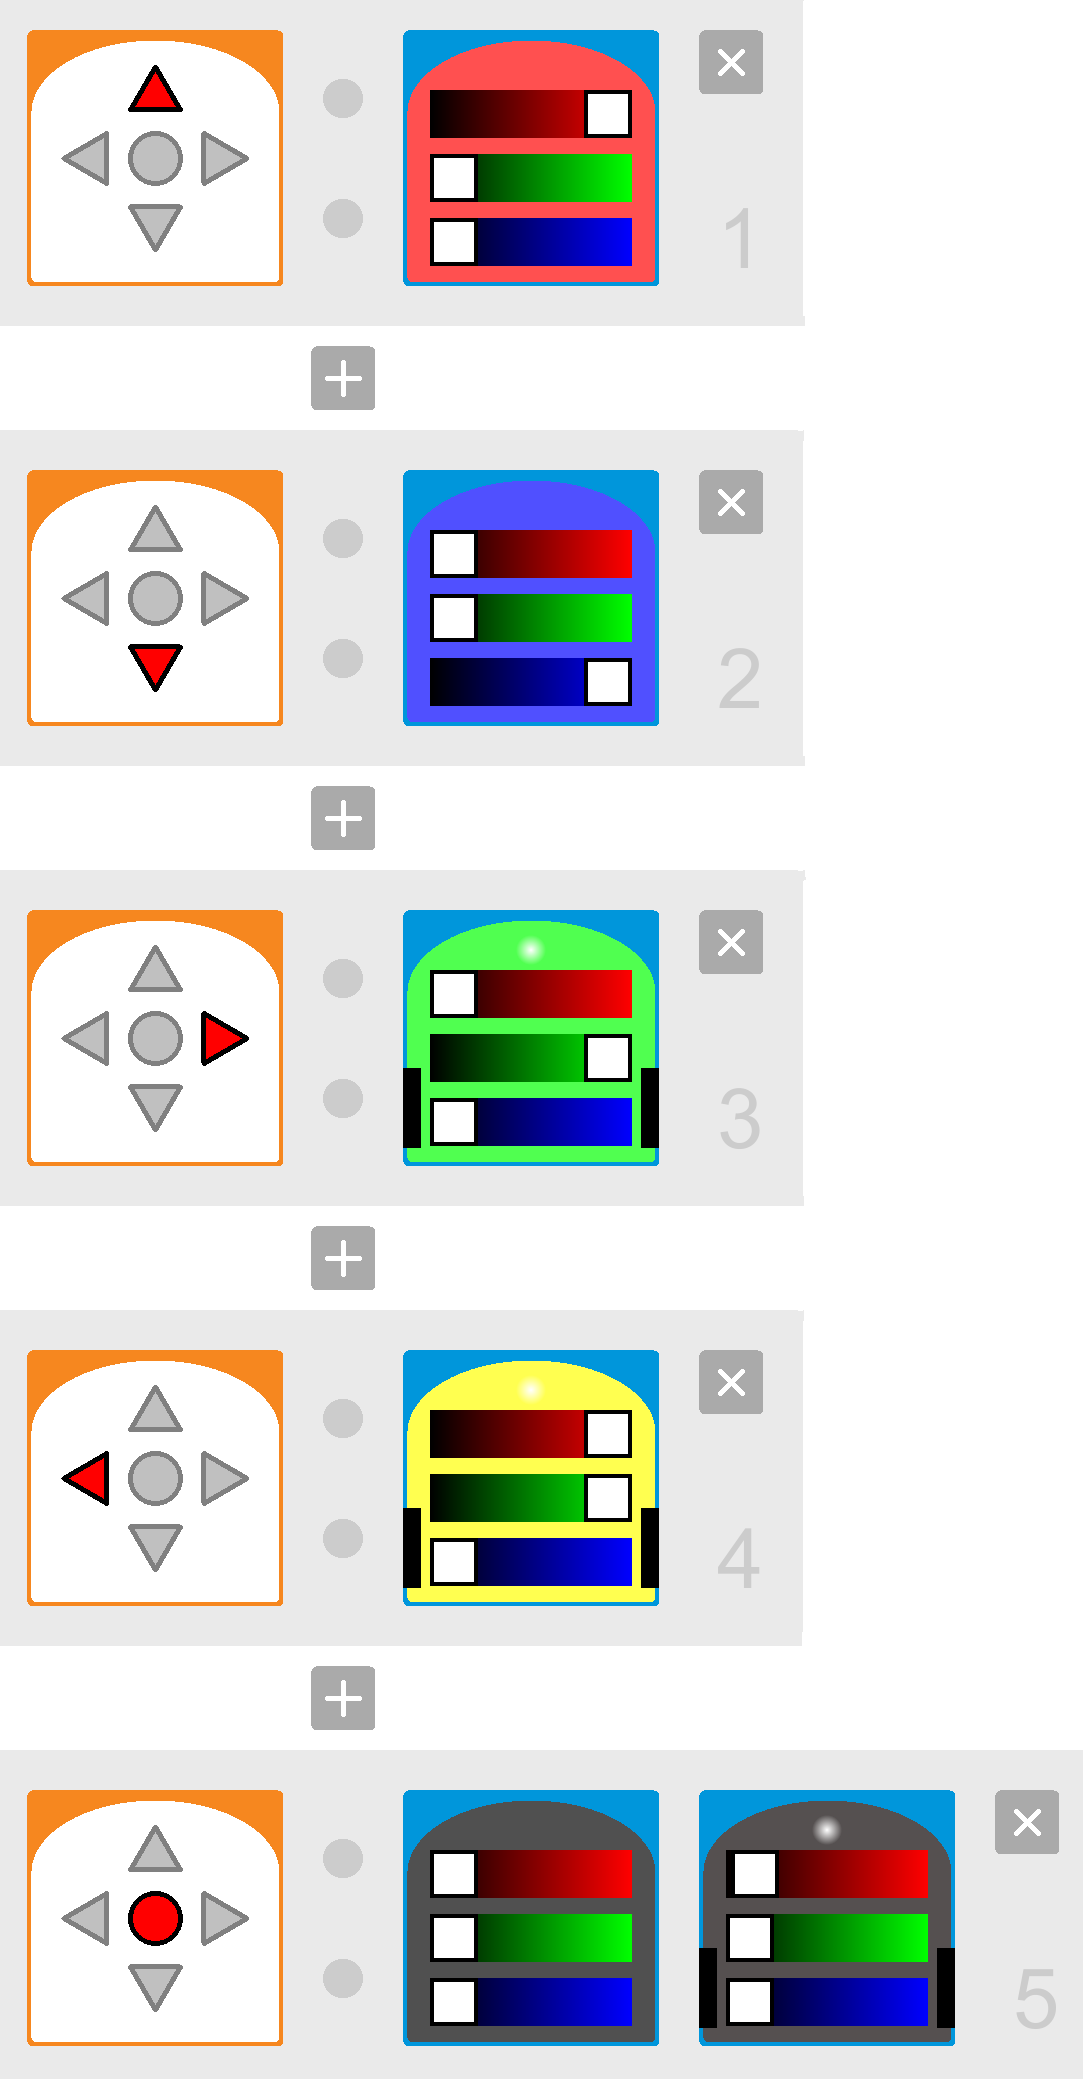
\includegraphics[width=.4\textwidth]{colors-multiple-full} &
\begin{minipage}[b]{.5\textwidth}
\begin{footnotesize}
\begin{verbatim}
  onevent buttons
    when button.forward == 1 do
      call leds.top(32,0,0)
    end
    when button.backward == 1 do
      call leds.top(0,0,32)
    end
    when button.right == 1 do
      call leds.bottom.left(0,32,0)
      call leds.bottom.right(0,32,0)
    end
    when button.left == 1 do
      call leds.bottom.left(32,32,0)
      call leds.bottom.right(32,32,0)
    end
    when button.center == 1 do
      call leds.top(0,0,0)
      call leds.bottom.left(7,0,0)
      call leds.bottom.right(7,0,0)
    end
\end{verbatim}
\end{footnotesize}
\vspace*{5ex}
\end{minipage}
\end{tabular}
\end{center}

In the AESL program, a \emph{single} event occurs when any of the five
buttons is touched. The action of the event handler \p{onevent buttons}
depends on which button is touched, so we check the value of the
\emph{button variables} in order to select an action. The statements:

\begin{footnotesize}
\begin{verbatim}
  when button.forward == 1 do
    call leds.top(32,0,0)
  end
\end{verbatim}
\end{footnotesize}

mean: \emph{when} the value of the variable \p{button.forward} changes
from some other value (here, 0) to 1, \emph{then} perform the actions
written on the lines between the keyword \p{do} and the keyword \p{end}.
There are five \p{button} variables, one for each button. The value of a
button variable is 1 if the button is touched and 0 if the button is
released. In the program, there are five \p{when}-statements, one for
each button. One or two actions are run if the expression in a
\p{when}-statement \emph{becomes} true.

\textbf{\large One event or multiple events$^*$}

The Thymio interface includes separate events for each button, in
addition to the \p{buttons} event that occurs if any button is touched
or released. We could implement the program as follows, using multiple
events without \p{when}-statements and button variables:

\begin{footnotesize}
\begin{verbatim}
  onevent button.forward
    call leds.top(32,0,0)
  
  onevent button.backward
    call leds.top(0,0,32)
  
  onevent button.right
    call leds.bottom.left(0,32,0)
    call leds.bottom.right(0,32,0)
  
  onevent button.left
    call leds.bottom.left(32,32,0)
    call leds.bottom.right(32,32,0)
  
  onevent button.center
    call leds.top(0,0,0)
    call leds.bottom.left(1,0,0)
    call leds.bottom.right(1,0,0)
\end{verbatim}
\end{footnotesize}

The advantage of using separate events is that the program is easier to
read and understand, but there are cases where you need to use the event
\p{buttons}: (a) to distinguish between touching and releasing a button,
and (b) to identify touching two buttons at once:

\begin{footnotesize}
\begin{verbatim}
  onevent buttons
    # Turn the top LEDs on when the forward button is released
    when button.forward == 0 do
      call leds.top(32,0,0)
    end

    # Turn the bottom LEDs on when
    #   both the left and the right buttons are  touched
    when button.left == 1 and button.right == 1 do
      call leds.bottom.left(0,32,0)
      call leds.bottom.right(0,32,0)
    end
\end{verbatim}
\end{footnotesize}


Another difference is that the individual events occur when a button is
touched or released, whereas the common event \p{buttons} occurs with a
frequency of 20 Hz after updating the array of button variables (see
page~\pageref{pg.hz} for an explanation of these concepts).


\textbf{\large \p{if}-statements}

AESL supports two alternative statements:
\begin{footnotesize}
\begin{verbatim}
  when v == 1 do ... statements ... end

  if v == 1 then ... statements ... end
\end{verbatim}
\end{footnotesize}
that have different meanings:
\begin{quote}
\emph{when} the value of \p{v} \emph{becomes} 1, run the statements

\emph{if} the value of \p{v} \emph{is} 1, run the statements
\end{quote}

\p{when}-statements are commonly used with variables representing
events, because we usually want to run an event handler when something
changes, not just because the value of a variable has a certain value.
We could write a \p{buttons} event handler using an \p{if}-statement:

\begin{footnotesize}
\begin{verbatim}
  onevent buttons
    if button.forward == 1 then
      ... statements ...
    end
\end{verbatim}
\end{footnotesize}
However, if we touch the forward button for a long period of time,
the statements would be run several times. If the statements change the
color of the LEDs, it wouldn't make a difference, but there are cases
where it does matter and a \p{when}-statement is needed.

An \p{if}-statement is appropriate when we are interested the values of
variables and not in their changes. The following statements set the
value of the variable \p{max} to the maximum value returned by the two
rear sensors:

\begin{footnotesize}
\begin{verbatim}
  if prox.horizontal[5] > prox.horizontal[6] then
    max = prox.horizontal[5]
  else
    max = prox.horizontal[6]
  end
\end{verbatim}
\end{footnotesize}

Additional examples of \p{if}-statements appear in the next section and
in Figure~\ref{fig.respond}.


\newpage

\sect{Arrays}

The program \p{likes.aesl} in \cref{ch.pet} of the VPL tutorial causes the
robot to follow your hand as you move it from side to side near the
forward horizontal proximity sensors.
When an object is not detected, the robot stops; when an object is
detected in front of the center sensor, the robot moves forward; when an
object is detected in front of the leftmost or rightmost sensor, the
robot turns in that direction.

\begin{figure}[hbt]
\begin{center}
\begin{tabular}{lr}
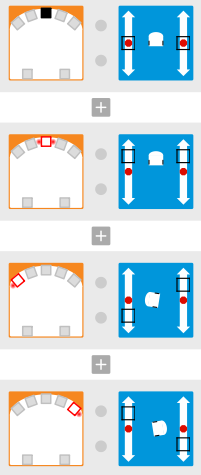
\includegraphics[width=.35\textwidth]{likes} &
\begin{minipage}[b]{.4\textwidth}
\begin{footnotesize}
\begin{verbatim}
  onevent prox
    when prox.horizontal[2] < 1000 do
      motor.left.target = 0
      motor.right.target = 0
    end
    when prox.horizontal[2] > 2000 do
      motor.left.target = 300
      motor.right.target = 300
    end
    when prox.horizontal[0] > 2000 do
      motor.left.target = -300
      motor.right.target = 300
    end
    when prox.horizontal[4] > 2000 do
      motor.left.target = 300
      motor.right.target = -300
    end
\end{verbatim}
\end{footnotesize}
\end{minipage}
\end{tabular}
\caption{The \p{likes} program in VPL and AESL}\label{fig.arrays}
\end{center}
\end{figure}

The AESL program (\cref{fig.arrays}) is structured as an event handler
with several \p{when}-statements. The values of the motor variables
\p{motor.left.target} and \p{motor.right.target} are set to values
corresponding to the positions of the sliders in the motor blocks. In
VPL, the sliders change the values of the motor variables in increments
of $50$, but in AESL you can set them to any values in the range $-500$
to $500$.

The event is called \p{prox}. Unlike the button events, which
occur when something ``happens,'' this event occurs \emph{10 times
>>>>>>> d0c474117e88c10d57f1a02945d63994237a9e8e
every second}. Before the event occurs, the values of the
\p{prox.horizontal} variables are set to values that depend on what the
sensors are detecting. See the\label{pg.hz} documentation of the
Thymio programming interface for details.\footnote{The unit
for \emph{frequency}, the number of times something happens per second, is called
the \emph{hertz}, abbreviated \emph{Hz}. The interface document specifies
that the {\footnotesize\p{prox}} event occurs with frequency \emph{10 Hz}.}

\textbf{\large Arrays as multiple variables}

The Thymio robot has 7 horizontal proximity sensors, 5 in front and 2 in
the back. To read the values detected by the sensors, it would be
possible to define 7 different variables:

\begin{footnotesize}
\begin{verbatim}
  prox.horizontal.front.0
  prox.horizontal.front.1
  prox.horizontal.front.2
  prox.horizontal.front.3
  prox.horizontal.front.4
  prox.horizontal.back.0
  prox.horizontal.back.1
\end{verbatim}
\end{footnotesize}

Instead, AESL enables you to define an \emph{array}, which is a sequence
of variables all with the same name. The different variables in the
sequence are identified with a number. The array for the horizontal
proximity sensors is predefined and is called \p{prox.horizontal}:

\begin{center}
\begin{picture}(240,40)
\put(0,0){\makebox(100,20)[l]{\p{prox.horizontal}}}
\put(100,0){\framebox(140,20){}}
\multiput(120,0)(20,0){6}{\line(0,1){20}}
\put(100,20){\makebox(20,20){\p{0}}}
\put(120,20){\makebox(20,20){\p{1}}}
\put(140,20){\makebox(20,20){\p{2}}}
\put(160,20){\makebox(20,20){\p{3}}}
\put(180,20){\makebox(20,20){\p{4}}}
\put(200,20){\makebox(20,20){\p{5}}}
\put(220,20){\makebox(20,20){\p{6}}}
\end{picture}
\end{center}

The first 5 components are for the front sensors from left to right,
while the last two components are for the back sensors from left to
right. If you don't remember the assignment of numbers to sensors, you
can always look it up in the the documentation for the Thymio
programming interface, even better, on the diagram in the reference
card.

To access a specific component in an array, write its sequence number in
square brackets after the name of the array variable. This number is
called an \emph{index} into the array. The following statement specifies
that the motor variables will be set to 300 when the value of the
\emph{front center sensor} (index 2) becomes greater than 2000:

\begin{footnotesize}
\begin{verbatim}
  when prox.horizontal[2] > 2000 do
    motor.left.target = 300
    motor.right.target = 300
  end
\end{verbatim}
\end{footnotesize}

Later, we will see that array variables can have their
values set in an assignment statement:
\begin{footnotesize}
\begin{verbatim}
  timer.period[0] = 1979
\end{verbatim}
\end{footnotesize}

\textbf{\large \p{for}-loops and index variables$^*$}

A natural generalization of arrays is to use a variable instead of a
constant for the index.\footnote{This is not used in translations of VPL
programs into AESL, except in an advanced construct for constructing
sounds; therefore, the simple example here is taken from the AESL
projects.} The program \p{cats.aesl} contains the following statements:

\begin{footnotesize}
\begin{verbatim}
  var i

  for i in 0:4 do
    if prox.horizontal[i] > DETECTION then
      state = 2
    end
  end
\end{verbatim}
\end{footnotesize}

Previously, we only used variables that are built into the Thymio
interface; here, the first line \emph{declares} a new variable called
\p{i}. The next statement is a \p{for}-statement whose meaning is:

\begin{itemize}
\item Assign the values 0, 1, 2, 3, 4 in turn to the variable \p{i};
\item For each assignment, run the statements between \p{do} and \p{end}.
\end{itemize}

Here, there is a single \p{if}-statement between \p{do} and \p{end}. It
checks the value of the horizontal proximity sensors and sets the value
2 in the variable \p{state} if the value read from a sensor is greater
than the constant \p{DETECTION}.\footnote{See the documentation of the 
Aseba Studio environment for instructions on how to define constants.}

The variable \p{i} receives the values 0, 1, 2, 3, 4 in turn, so each
time the \p{if}-statement is run, \p{prox.horizontal[i]} reads the value
of each front sensor from left to right. The result of the
\p{for}-statement is thus to set the value of the variable \p{state} to
2 \emph{if} \emph{any} of the front sensors detects an object.

\textbf{\large Declaring an array}

An array variable is declared by giving its size in brackets following
the array name. The size can also be specified by providing an initial
value:\footnote{A comment need not start at the beginning of a line.
Every character from the symbol \# to the end of the line is considered
to be a comment and is ignored by the computer.} 

\begin{footnotesize}
\begin{verbatim}
var state[4]             # An array with four components
var state[] = [0,0,0,0]  # An array with four components
\end{verbatim}
\end{footnotesize}

In the translation of the VPL program, both the size and the initial
value are given. This is correct as long as the number of values is the
same as the size:

\begin{footnotesize}
\begin{verbatim}
var state[4] = [0,0,0,0]  # OK, but redundant
\end{verbatim}
\end{footnotesize}

\newpage

\sect{Timers}

\cref{ch.time} introduced \emph{timers}. The program
\p{shy.aesl} causes the robot to turn left when the front center sensor
detects your hand; two seconds later, it turns right:

\begin{center}
\begin{tabular}{ll}
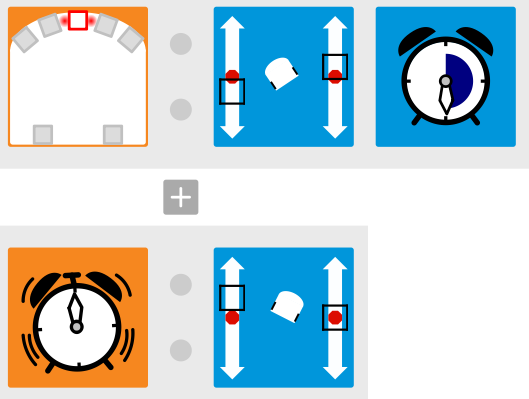
\includegraphics[width=.4\textwidth]{shy} &
\begin{minipage}[b]{.5\textwidth}
\begin{footnotesize}
\begin{verbatim}
  onevent prox
    when prox.horizontal[2] > 2000 do
      motor.left.target = -150
      motor.right.target = 100
      timer.period[0] = 2000
    end
  
  onevent timer0
    timer.period[0] = 0
    motor.left.target = 200
    motor.right.target = 0
\end{verbatim}
\end{footnotesize}
%\vspace*{1ex}
\end{minipage}
\end{tabular}
\end{center}

There are two timers in the Thymio robot. You set the duration of a
timer by assigning a value to components 0 or 1 of the array
\p{timer.period}. The value is in \emph{milliseconds}, thousandths of a
second. To set a duration of 2 seconds in timer 0, the value 2000
(milliseconds) should be assigned to \p{timer.period[0]}.

There are two events, \p{timer0} and \p{timer1}, one for each timer.
When the duration has passed (we say that the timer has \emph{expired}),
the timer event occurs. In the handler for the event \p{timer0}, we set
the timer duration to 0 so it won't occur again and change the motor
settings.

As part of its initialization, the program sets the timer to 0 so that
the event won't accidently occur at the beginning of the program:

\begin{footnotesize}
\begin{verbatim}
  # stop timer 0
  timer.period[0] = 0
\end{verbatim}
\end{footnotesize}

\newpage

\sect{States}

\cref{ch.states,ch.counting} showed how to use \emph{states}. The
Thymio robot can be in one of 16 states and you can specify that an
event causes an action only if the robot is in certain states. In the
program \p{count-to-two.aesl} from \cref{ch.counting}, the state is set to 0 when
the center button is touched and then it counts whether the number of
claps is even or odd by alternating between state 0 and state 1. The VPL
program and the AESL event handler for touching the center button
are:\footnote{The AESL program shown here is different from the one
generated by VPL as explained later in this chapter.}

\begin{center}
\begin{tabular}{ll}
\raisebox{8ex}{
\includegraphics[width=.4\textwidth]{two-button}} &
\begin{minipage}[b]{.5\textwidth}
\begin{footnotesize}
\begin{verbatim}
  var state[] = [0,0,0,0]
  
  onevent buttons
    when button.center == 1 do
      state[0] = 0
      state[1] = 0
      state[2] = 0
      state[3] = 0
    end
\end{verbatim}
\end{footnotesize}
\end{minipage}
\end{tabular}
\end{center}

The state is stored in an array \p{state[]} which has 4 components. Each
component can be 0 or 1, so there are $2\times 2\times 2\times 2=16$
possible values in the array. The components of the array are given
initial values of 0 by assigning the four values
{\footnotesize\verb+[0,0,0,0]+}. The initial value of the array is also
used to specify the number of components in an array; since there are 4
values in {\footnotesize\verb+[0,0,0,0]+}, there are 4 components in the
array.

The state event block (green, next to the button event block) has all of
its quarters set to gray; this means that the event can occur regardless
of the current value of the state. Therefore, whenever the center button
is touched, the state action block (blue) causes all the components of
the array \p{state} to be set to 0, as indicated by the white quarters.
In the corresponding AESL program, the \p{if}-statement checks if the
button was touched, but does not check the value of the array \p{state}.
If the button was touched, each component of the array is set to 0.

There are two clap event blocks, each one associated with a different
state block. In the textual program a single \p{mic} event handler will
be used. The statements to be run will depend on \p{if}-statements
(\cref{fig.respond}).

\begin{figure}[hbt]
\begin{center}
\begin{tabular}{ll}
\raisebox{10ex}{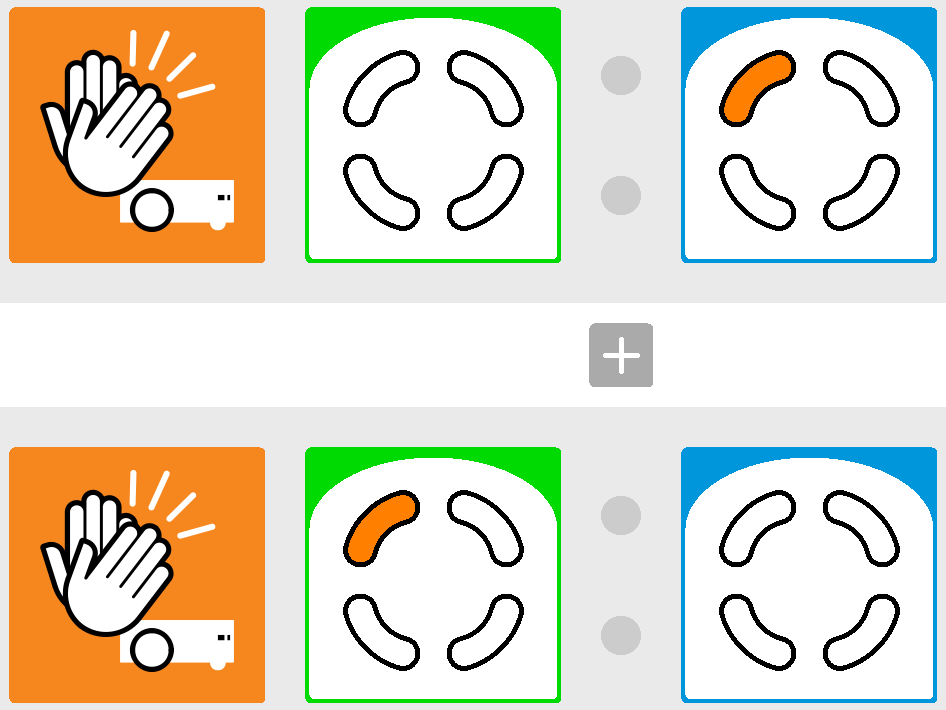
\includegraphics[width=.4\textwidth]{two-clap}} &
\begin{minipage}[b]{.5\textwidth}
\begin{footnotesize}
\begin{verbatim}
  onevent mic
    if state[0] == 0 and
       state[1] == 0 and
       state[2] == 0 and
       state[3] == 0 then
      state[0] = 1
      state[1] = 0
      state[2] = 0
      state[3] = 0
    end
    if state[0] == 1 and
       state[1] == 0 and
       state[2] == 0 and
       state[3] == 0 then
      state[0] = 0
      state[1] = 0
      state[2] = 0
      state[3] = 0
    end
\end{verbatim}
\end{footnotesize}
\end{minipage}
\end{tabular}
\caption{Responding to claps according to the state}\label{fig.respond}
\end{center}
\end{figure}

The meaning of the keyword \p{and} is that \emph{all} the conditions in
the \p{if}-statement must hold in order to run the statements between
\p{then} and \p{end}. If all components of \p{state} are 0, the value of
\p{state[0]} is set to 1, while the others are set to 0. This
corresponds to the state event block having all quarters white and the
state action block having the upper left quarter orange and the others
white. Similarly, if value of \p{state[0]} is 1 and the values of the
other components are 0, the values of all the components of \p{state}
are set to 0.

\newpage

\sect{Subroutines}

Quite often we need to run the same sequence of statements from many
places within a program. We could write the statements once and copy
them each time they are needed. A simpler solution is to use a
\emph{subroutine}, which assigns a name to a sequence of statements. In
this program, the declaration {\footnotesize\verb+sub display_state+}
declares a subroutine that assigns the name
{\footnotesize\verb+display_state+} to a sequence of statements, here,
the single statement \p{call leds.circle}:

\begin{footnotesize}
\begin{verbatim}
  # subroutine to display the current state
  sub display_state
    call leds.circle(
      0, state[1]*32, 0, state[3]*32, 0, state[2]*32, 0, state[0]*32)
\end{verbatim}
\end{footnotesize}

When the subroutine is \emph{called}, it runs the statements assigned to
the name of the subroutine:
\vspace{-1ex}
\begin{footnotesize}
\begin{verbatim}
  callsub display_state
\end{verbatim}
\end{footnotesize}
\vspace{-1ex}
The interface function \p{leds.circle} sets the eight curved LEDs
surrounding the buttons. You really do need to refer to the cheat sheet
to learn which parameter sets which LED!

The intensity of each LED is set by giving the corresponding parameter a
value between 0 (off) and 32 (full intensity). The front, back,
left and right LEDs are set to 0 (off), whereas the diagonal LEDs are
set to on if the corresponding state component is 1 and off if the state
component is 0. This is achieved by the \emph{arithmetic expressions}
\p{state[...]*32} which multiply the value of the components of the array
by 32. If one of the values is 0, the result is 0, while if it is 1, the
result is 32.

\newpage

\sect{Native functions}

The program above has a problem. Since the components of the array
\p{state} are set one-by-one, it is possible that an different event
will occur when some, but not all, of the components have been set. To
set all the components at once, the new values of the state are first
set in a second array \p{new\_state} and then they are copied to the
first array \p{state}:

\begin{footnotesize}
\begin{verbatim}
# variables for state
var state[4] = [0,0,0,0]
var new_state[4] = [0,0,0,0]

onevent buttons
  when button.center == 1 do
    new_state[0] = 0
    new_state[1] = 0
    new_state[2] = 0
    new_state[3] = 0
  end

  call math.copy(state, new_state)
  callsub display_state
\end{verbatim}
\end{footnotesize}

The \emph{native function} \p{math.copy} is used to copy the arrays.
Native functions are built into the Thymio robot and are more efficient
than sequences of statements in AESL. The native functions are described
in the Aseba documentation.

The current version of AESL allows assignment of entire arrays, so that
it would have been possible to use the assignment
statement:\footnote{The array assignment translates into a sequence of
individual assignment statements, one for each component, so nothing is
actually gained by using an array assignment statement.}

\begin{footnotesize}
\begin{verbatim}
  state = new_state
\end{verbatim}
\end{footnotesize}

\end{document}
